\documentclass[aspectratio=169]{beamer}

% Shared Beamer settings for Applied Machine Learning lectures (UPES).
% Keep this file free of \documentclass to allow reuse via \input.

% Allow lecture sources to use shared theme/assets without copying them into each lecture folder.
% NOTE: These paths are relative to `Unit-xx/Lecture-yy/latex/` (and `Lab/Experiment-xx/latex/`).
\makeatletter
\def\input@path{{../../../_shared/}{../../../_shared/UPES-Beamer-Theme/}}
\makeatother

\usetheme{UPES}
\setbeamertemplate{navigation symbols}{}

\usepackage{amsmath}
\usepackage{amssymb}
\usepackage{booktabs}
\usepackage{graphicx}
\usepackage{hyperref}
\usepackage{xcolor}
\usepackage{listings}

% Code listings (Python-oriented for this subject).
\lstset{
  language=Python,
  basicstyle=\ttfamily\small,
  keywordstyle=\color{blue},
  commentstyle=\color{gray},
  stringstyle=\color{teal},
  showstringspaces=false,
  columns=fullflexible,
  breaklines=true
}

\usepackage{tikz}
\usetikzlibrary{arrows.meta,positioning,shapes.geometric,calc,fit,backgrounds}

% Per-slide source line (references shown on the slide itself).
\newcommand{\slidesources}[1]{%
  \vfill
  {\tiny\color{gray}\raggedright\sloppy\parbox{\linewidth}{Sources: #1}\par}%
}

% Unit-wise source strings for this subject (used by slides/notes).
% Path is relative to the lecture `latex/` folder (the compilation CWD).
% Source strings for Applied Machine Learning (CSAI2017P) — used by slides + notes.
% Prescribed texts and reference books are taken from the course syllabus.
% Support texts are the author-hosted open-access editions:
%   statlearning.com            (ISL with Python)
%   probml.github.io/pml-book   (Murphy, Probabilistic Machine Learning)
%   d2l.ai                      (Dive into Deep Learning)
%   mml-book.github.io          (Mathematics for Machine Learning)

\newcommand{\AMLRepoURL}{https://github.com/tali7c/Applied-Machine-Learning}

% --- prescribed -------------------------------------------------------------
\newcommand{\AMLPrescribed}{%
M\"uller and Guido, \textit{Introduction to Machine Learning with Python}, O'Reilly, 2016.;%
Bishop, \textit{Pattern Recognition and Machine Learning}, Springer, 2006.;%
Murphy, \textit{Machine Learning: A Probabilistic Perspective}, MIT Press, 2012.;%
Han, Kamber and Pei, \textit{Data Mining: Concepts and Techniques} (3e), Morgan Kaufmann, 2012.%
}

% --- unit-wise ---------------------------------------------------------------
\newcommand{\AMLUnitISources}{%
M\"uller and Guido, \textit{Introduction to Machine Learning with Python}, Ch. 1.;%
Bishop, \textit{Pattern Recognition and Machine Learning}, Ch. 1.;%
Murphy, \textit{Probabilistic Machine Learning: An Introduction}, MIT Press, 2022, Ch. 1.;%
Mitchell, \textit{Machine Learning}, McGraw Hill, 1997, Ch. 1.;%
Scikit-learn documentation, accessed 2026-08-04.%
}

\newcommand{\AMLUnitIISources}{%
Bishop, \textit{Pattern Recognition and Machine Learning}, \S1.5, \S4.3, \S7.1.;%
Zhang, Lipton, Li and Smola, \textit{Dive into Deep Learning}, \S3.4.;%
Shalev-Shwartz and Ben-David, \textit{Understanding Machine Learning}, Ch. 15.;%
Murphy, \textit{Probabilistic Machine Learning: An Introduction}, Ch. 5.%
}

\newcommand{\AMLUnitIIISources}{%
Zhang, Lipton, Li and Smola, \textit{Dive into Deep Learning}, Ch. 12 (Optimization Algorithms).;%
Deisenroth, Faisal and Ong, \textit{Mathematics for Machine Learning}, Ch. 7.;%
Kingma and Ba, ``Adam: A Method for Stochastic Optimization,'' ICLR 2015.;%
Ruder, ``An overview of gradient descent optimization algorithms,'' arXiv:1609.04747, 2016.%
}

\newcommand{\AMLUnitIVSources}{%
Han, Kamber and Pei, \textit{Data Mining: Concepts and Techniques} (3e), Ch. 3.;%
M\"uller and Guido, \textit{Introduction to Machine Learning with Python}, Ch. 3--4.;%
James, Witten, Hastie, Tibshirani and Taylor, \textit{An Introduction to Statistical Learning with Python}, Ch. 5--6, 12.;%
Scikit-learn documentation (preprocessing, model selection), accessed 2026-08-04.%
}

\newcommand{\AMLUnitVSources}{%
James et al., \textit{An Introduction to Statistical Learning with Python}, Ch. 3--6.;%
Bishop, \textit{Pattern Recognition and Machine Learning}, Ch. 3.;%
Deisenroth, Faisal and Ong, \textit{Mathematics for Machine Learning}, Ch. 9.;%
M\"uller and Guido, \textit{Introduction to Machine Learning with Python}, \S2.3.%
}

\newcommand{\AMLUnitVISources}{%
Han, Kamber and Pei, \textit{Data Mining: Concepts and Techniques} (3e), Ch. 8--9.;%
James et al., \textit{An Introduction to Statistical Learning with Python}, Ch. 8--9.;%
Bishop, \textit{Pattern Recognition and Machine Learning}, Ch. 4--5, 7, 14.;%
Zhang et al., \textit{Dive into Deep Learning}, Ch. 5.%
}

\newcommand{\AMLUnitVIISources}{%
Han, Kamber and Pei, \textit{Data Mining: Concepts and Techniques} (3e), Ch. 10.;%
James et al., \textit{An Introduction to Statistical Learning with Python}, Ch. 12.;%
M\"uller and Guido, \textit{Introduction to Machine Learning with Python}, \S3.5.;%
Ester, Kriegel, Sander and Xu, ``A density-based algorithm for discovering clusters (DBSCAN),'' KDD 1996.%
}

\newcommand{\AMLLabSources}{%
M\"uller and Guido, \textit{Introduction to Machine Learning with Python}, companion notebooks.;%
McKinney, \textit{Python for Data Analysis} (3e), O'Reilly, 2022.;%
Scikit-learn user guide, accessed 2026-08-04.;%
Matplotlib and Seaborn documentation, accessed 2026-08-04.%
}



\graphicspath{{../figures/}{../images/}{../../../_shared/}{../../../_shared/UPES-Beamer-Theme/}}

\title[Applied Machine Learning]{Applied Machine Learning}
\subtitle{Unit 07 -- Lecture 23: Partitioning and Density-Based Clustering}
\author{Tofik Ali}
\institute{School of Computer Science, UPES Dehradun}
\date{Autumn 2026}

% ---- a compact "output" block so code and its result sit together ----------
\lstdefinestyle{outblk}{
  basicstyle=\ttfamily\scriptsize\color{black!75},
  backgroundcolor=\color{black!5}, frame=leftline, framerule=2pt,
  rulecolor=\color{black!30}, breaklines=true, columns=fullflexible,
  keepspaces=true,   % several outputs below are aligned tables
  language={},       % printed output is not Python: do not syntax-highlight it
  xleftmargin=4pt, aboveskip=1pt, belowskip=1pt, literate={-}{{-}}1}
\lstnewenvironment{outblk}{\lstset{style=outblk}}{}

\begin{document}

\UPESCoverFrame
\setcounter{framenumber}{0}

\begin{frame}[shrink=5]
  \titlepage
  \begin{center}
    \footnotesize Choose $k$ representatives. Assign. Repeat.\\[0.25em]
    \footnotesize Topic focus: \textbf{what a ``cluster centre'' is}\\[0.25em]
    \footnotesize Repository: \texttt{\AMLRepoURL}
  \end{center}
  \slidesources{\AMLUnitVIISources}
\end{frame}

\begin{frame}{Quick Links}
  \centering
  \hyperlink{sec:part}{\beamerbutton{Partitioning}}\hspace{0.4em}
  \hyperlink{sec:hand}{\beamerbutton{$k$-means by hand}}\hspace{0.4em}
  \hyperlink{sec:conv}{\beamerbutton{Convergence}}\hspace{0.4em}
  \hyperlink{sec:k}{\beamerbutton{Choosing $k$}}\\[0.6em]
  \hyperlink{sec:assume}{\beamerbutton{Assumptions}}\hspace{0.4em}
  \hyperlink{sec:medoid}{\beamerbutton{$k$-medoids / PAM}}\hspace{0.4em}
  \hyperlink{sec:clara}{\beamerbutton{CLARA}}\\[0.6em]
  \hyperlink{sec:dbscan}{\beamerbutton{DBSCAN}}\hspace{0.4em}
  \hyperlink{sec:eps}{\beamerbutton{One global eps}}\hspace{0.4em}
  \hyperlink{sec:summary}{\beamerbutton{Summary}}
\end{frame}

\begin{frame}{Agenda}
  \tableofcontents
\end{frame}

\begin{frame}[shrink=8]{How this lecture works}
  \begin{columns}[T]
    \begin{column}{0.48\textwidth}
      \begin{block}{Every idea appears twice}
        \begin{enumerate}
          \item \textbf{By hand} --- seven points and a pen for $k$-means,
            eleven points and a pen for DBSCAN. Small enough that every
            number can be checked.
          \item \textbf{In code} --- the same numbers out of
            \texttt{sklearn.cluster}, agreeing exactly, so you can see the
            library is doing precisely this and nothing magic.
        \end{enumerate}
      \end{block}
    \end{column}
    \begin{column}{0.48\textwidth}
      \begin{alertblock}{Commit before you look}
        Seven slides ask you to predict something before it is revealed.
        Write your guess down. Being wrong on paper is how the idea sticks.
      \end{alertblock}
    \end{column}
  \end{columns}
  \vspace{0.4em}
  \begin{center}
    \small Two calculations carry the lecture: \textbf{a complete $k$-means
    run on seven points, iteration by iteration, with the objective written
    down after every half step}, and \textbf{eleven points labelled core,
    border or noise arithmetically}. Those are the examinable ones.
  \end{center}
\end{frame}

\begin{frame}[shrink=6]{Three kinds of seed --- this lecture uses all three}
  \begin{columns}[T]
    \begin{column}{0.32\textwidth}
      \begin{block}{One arbitrary seed}
        \small \textbf{0}. Any \texttt{KMeans} start that is not an
        experiment, every CLARA run, every contamination draw.
      \end{block}
    \end{column}
    \begin{column}{0.32\textwidth}
      \begin{block}{Dataset seeds}
        \small \texttt{random\_state=7} (six blobs), \texttt{11} (four
        clean), \texttt{3} (unequal sizes). These fix the \emph{shape} ---
        and the shape is the argument.
      \end{block}
    \end{column}
    \begin{column}{0.32\textwidth}
      \begin{block}{Sweep seeds}
        \small \texttt{for s in range(200)}. The disagreement between runs
        \emph{is} the result. Collapse it and you delete the lecture.
      \end{block}
    \end{column}
  \end{columns}
  \vspace{0.4em}
  \begin{alertblock}{Pin \texttt{n\_init} as well as \texttt{random\_state}}
    \centering\small
    \texttt{random\_state} fixes \emph{where} the starts come from;
    \texttt{n\_init} fixes \emph{how many}. Its default is
    \texttt{"auto"} --- $1$ for \texttt{k-means++}, $10$ for
    \texttt{init="random"} --- and it changed in scikit-learn~1.4. Write
    \texttt{KMeans(n\_clusters=6)} alone and you will not reproduce these
    figures.
  \end{alertblock}
\end{frame}

\begin{frame}[shrink=6]{Where we are}
  \begin{columns}[T]
    \begin{column}{0.47\textwidth}
      \begin{block}{The last lecture}
        Hierarchical clustering: you supply nothing, you get a tree, you
        choose $k$ afterwards. It is deterministic and it never undoes a
        merge --- and it needs $O(n^2)$ memory, so it stops at a few tens of
        thousands of rows.
      \end{block}
    \end{column}
    \begin{column}{0.49\textwidth}
      \begin{exampleblock}{Today: the other bargain}
        \textbf{Partitioning.} You supply $k$. You get one partition, fast,
        on data a hierarchy could not touch --- and you get a
        \emph{different} answer every run.
      \end{exampleblock}
      \begin{alertblock}{And then: refuse the bargain}
        \textbf{Density-based.} Do not supply $k$, do not assume round
        clusters, and let the method say ``this point belongs to nothing''.
      \end{alertblock}
    \end{column}
  \end{columns}
\end{frame}

% =====================================================================
\section[Partitioning]{Partitioning: the problem and the objective}
\label{sec:part}

\begin{frame}[shrink=10]{The partitioning problem, stated precisely}
  \begin{block}{Given}
    $n$ objects and an integer $k$. \textbf{Find} a partition into exactly
    $k$ non-empty groups that optimises some criterion.
  \end{block}
  \begin{exampleblock}{The criterion for $k$-means: within-cluster sum of squares}
    \centering\large
    $\displaystyle
      \mathrm{WCSS} = \sum_{j=1}^{k} \sum_{x \in C_j}
      \lVert x - c_j \rVert_2^2,
      \qquad c_j = \frac{1}{|C_j|}\sum_{x \in C_j} x$
  \end{exampleblock}
  \begin{columns}[T]
    \begin{column}{0.49\textwidth}
      \begin{block}{Three names for the same number}
        \small $\mathrm{WCSS}$, \emph{inertia} (scikit-learn's
        \texttt{inertia\_}), and the \emph{distortion}. All the same sum.
      \end{block}
    \end{column}
    \begin{column}{0.49\textwidth}
      \begin{alertblock}{Note the square}
        \small $k$-means minimises \emph{squared} Euclidean distance. That is
        not a detail --- it is exactly why the optimal representative of a
        cluster is its \textbf{mean}, and why one far-away point costs so
        much.
      \end{alertblock}
    \end{column}
  \end{columns}
\end{frame}

\begin{frame}[fragile,shrink=8]{Why not just try all the partitions?}
\begin{outblk}
   n      k    number of partitions S(n,k)
     7      2    63
    10      3    9330
    25      3    1.41198e+11
    50      5    7.40096e+32
   100      3    8.58963e+46
\end{outblk}
  \vspace{0.2em}
  \begin{columns}[T]
    \begin{column}{0.5\textwidth}
      \begin{block}{Stirling numbers of the second kind}
        \small
        $S(n,k) = \frac{1}{k!}\sum_{i=0}^{k}(-1)^i \binom{k}{i}(k-i)^n$.
        \\[0.3em]
        With $k = 2$ it is just $2^{n-1}-1$. On seven points that is $63$
        and we will check every one of them.
      \end{block}
    \end{column}
    \begin{column}{0.48\textwidth}
      \begin{alertblock}{$k$-means is NP-hard}
        \small Even for $k = 2$ in general dimension, and even for $d = 2$
        with general $k$. So we do not solve it. We run a heuristic, and we
        are honest that it is one.
      \end{alertblock}
    \end{column}
  \end{columns}
  \vspace{0.2em}
  \begin{center}\small
    But the number \emph{is} finite --- hold that thought, it is half the
    convergence proof.
  \end{center}
\end{frame}

\begin{frame}[fragile,shrink=10]{Lloyd's algorithm, in eight lines}
\begin{lstlisting}[language=]
Input : n points, an integer k, initial centroids c_1 ... c_k
Output: an assignment of every point to one of k clusters

repeat
    # ASSIGNMENT step
    for each point x:  assign x to the cluster j minimising ||x - c_j||
    # UPDATE step
    for each cluster j: c_j = mean of the points now assigned to j
until no point changes cluster
\end{lstlisting}
  \begin{columns}[T]
    \begin{column}{0.49\textwidth}
      \begin{exampleblock}{Two steps, alternating}
        \small Fix the centres, optimise the assignment. Fix the assignment,
        optimise the centres. Neither step ever needs to look at the other's
        problem.
      \end{exampleblock}
    \end{column}
    \begin{column}{0.49\textwidth}
      \begin{alertblock}{What is \emph{not} in the loop}
        \small No $k$-selection, no convergence tolerance, no learning rate.
        The only free choice is the \textbf{initial centroids} --- and that
        choice decides the answer.
      \end{alertblock}
    \end{column}
  \end{columns}
\end{frame}

% =====================================================================
\section[$k$-means by hand]{A complete $k$-means run, by hand}
\label{sec:hand}

\begin{frame}[shrink=6]{Seven points, $k = 2$, and a deliberately bad start}
  \begin{center}
    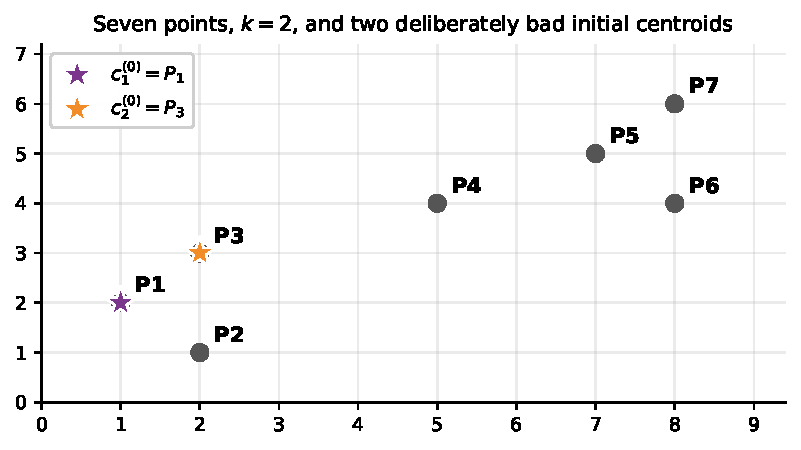
\includegraphics[width=0.72\textwidth]{handpoints.pdf}
  \end{center}
  \vspace{-0.3em}
  \begin{center}\small
    $P_1(1,2)\quad P_2(2,1)\quad P_3(2,3)\quad P_4(5,4)\quad P_5(7,5)\quad
     P_6(8,4)\quad P_7(8,6)$
    \\[0.2em]
    Initial centroids taken from the data:
    $c_1^{(0)} = P_1 = (1,2)$ and $c_2^{(0)} = P_3 = (2,3)$ --- both on the
    left, on purpose.
  \end{center}
\end{frame}

\begin{frame}{Predict first \#1 --- where will this end up?}
  \begin{alertblock}{Commit to an answer}
    Both starting centroids are in the left-hand clump. The four points on
    the right are nowhere near either of them.

    \medskip
    \centering\large
    Does $k$-means recover $\{P_1,P_2,P_3\}$ and $\{P_4,P_5,P_6,P_7\}$
    from that start? How many iterations?
  \end{alertblock}
  \onslide<2->{
  \begin{exampleblock}{}
    \centering\large
    \textbf{Yes} --- and in \textbf{three} iterations, with exactly
    \textbf{one} point changing cluster on the way.
  \end{exampleblock}
  \begin{center}\small
    The interesting part is \emph{which} point moves, and \emph{when}. At
    iteration 1 the split is $\{P_1,P_2\}$ against the other five. Watch
    $P_3$.
  \end{center}}
\end{frame}

\begin{frame}[fragile,shrink=6]{By hand, iteration 1 --- the assignment step}
  \begin{center}\small
    $c_1 = (1,2)$, $c_2 = (2,3)$. One Euclidean distance per point per
    centroid; assign to the smaller.
  \end{center}
\begin{outblk}
  point      coord      d(.,c1)   d(.,c2)   cluster
  P1     ( 1.0, 2.0)    0.0000    1.4142   C1
  P2     ( 2.0, 1.0)    1.4142    2.0000   C1
  P3     ( 2.0, 3.0)    1.4142    0.0000   C2
  P4     ( 5.0, 4.0)    4.4721    3.1623   C2
  P5     ( 7.0, 5.0)    6.7082    5.3852   C2
  P6     ( 8.0, 4.0)    7.2801    6.0828   C2
  P7     ( 8.0, 6.0)    8.0623    6.7082   C2
  clusters: C1 = {P1,P2}   C2 = {P3,P4,P5,P6,P7}
\end{outblk}
  \vspace{0.2em}
  \begin{center}\small
    $d(P_2,c_1) = \sqrt{1^2+1^2} = \sqrt{2} = 1.4142$ against
    $d(P_2,c_2) = \sqrt{0^2+2^2} = 2$. Every entry is checkable in your head.
    \\[0.2em]
    \textbf{WCSS after this assignment} $=\ 2 + 121 = \mathbf{123.0000}$.
  \end{center}
\end{frame}

\begin{frame}[fragile,shrink=8]{By hand, iteration 1 --- the update step}
  \begin{columns}[T]
    \begin{column}{0.52\textwidth}
      \begin{block}{New centroids are plain averages}
        \small
        $c_1 = \frac12\bigl((1{+}2),\ (2{+}1)\bigr) = (1.5,\ 1.5)$
        \\[0.3em]
        $c_2 = \frac15\bigl((2{+}5{+}7{+}8{+}8),\ (3{+}4{+}5{+}4{+}6)\bigr)$
        \\ \hspace{1.1em} $= \bigl(\tfrac{30}{5},\ \tfrac{22}{5}\bigr)
           = (6.0,\ 4.4)$
      \end{block}
    \end{column}
    \begin{column}{0.46\textwidth}
\begin{outblk}
  c1 = mean{P1,P2}       = (1.5, 1.5)
  c2 = mean{P3..P7}      = (6.0, 4.4)
  WCSS after assignment  = 123.0000
  WCSS after update      =  32.2000
\end{outblk}
    \end{column}
  \end{columns}
  \vspace{0.3em}
  \begin{exampleblock}{Check the drop by hand}
    \centering\small
    $C_1$ contributes $0.5 + 0.5 = 1.0$. $C_2$ contributes
    $17.96 + 1.16 + 1.36 + 4.16 + 6.56 = 31.2$. Total
    $\mathbf{32.2}$, down from $123$.
  \end{exampleblock}
  \begin{alertblock}{}
    \centering\small
    Nothing was reassigned. The objective fell by $90.8$ purely because the
    centres moved to the means. \textbf{That is what the update step is for.}
  \end{alertblock}
\end{frame}

\begin{frame}{Predict first \#2 --- does anything move now?}
  \begin{alertblock}{Commit to an answer}
    The centroids are now $c_1 = (1.5,\ 1.5)$ and $c_2 = (6.0,\ 4.4)$.
    $P_3$ sits at $(2,3)$ and is currently in $C_2$.

    \medskip
    \centering\large
    Does $P_3$ stay in $C_2$? Compute the two distances before you look.
  \end{alertblock}
  \onslide<2->{
  \begin{exampleblock}{}
    \centering\large
    $d(P_3,c_1) = \sqrt{0.25 + 2.25} = \mathbf{1.5811}$ \qquad
    $d(P_3,c_2) = \sqrt{16 + 1.96} = \mathbf{4.2379}$
    \\[0.3em]
    \textbf{$P_3$ moves to $C_1$}, and no other point changes.
  \end{exampleblock}
  \begin{center}\small
    $P_3$ was only in $C_2$ because $c_2$ \emph{started} on top of it. One
    update step later, $c_2$ has been dragged away to $(6, 4.4)$ by the four
    right-hand points, and $P_3$ is abandoned.
  \end{center}}
\end{frame}

\begin{frame}[fragile,shrink=8]{By hand, iterations 2 and 3}
  \begin{columns}[T]
    \begin{column}{0.52\textwidth}
      \begin{center}\small\textbf{Iteration 2: $P_3$ crosses over}\end{center}
\begin{outblk}
  point      coord      d(.,c1)  d(.,c2)  cl
  P1     ( 1.0, 2.0)    0.7071   5.5462   C1
  P2     ( 2.0, 1.0)    0.7071   5.2498   C1
  P3     ( 2.0, 3.0)    1.5811   4.2379   C1  <--
  P4     ( 5.0, 4.0)    4.3012   1.0770   C2
  P5     ( 7.0, 5.0)    6.5192   1.1662   C2
  P6     ( 8.0, 4.0)    6.9642   2.0396   C2
  P7     ( 8.0, 6.0)    7.9057   2.5612   C2
  WCSS after assignment = 16.7400
  c1 = mean{P1,P2,P3}   = (1.6667, 2.0000)
  c2 = mean{P4..P7}     = (7.0000, 4.7500)
  WCSS after update     = 11.4167
\end{outblk}
    \end{column}
    \begin{column}{0.46\textwidth}
      \begin{center}\small\textbf{Iteration 3: nothing moves}\end{center}
\begin{outblk}
  P1  0.6667  6.6002  C1
  P2  1.0541  6.2500  C1
  P3  1.0541  5.2974  C1
  P4  3.8873  2.1360  C2
  P5  6.1192  0.2500  C2
  P6  6.6416  1.2500  C2
  P7  7.4907  1.6008  C2
  no point changed cluster
  CONVERGED after 3 iterations
\end{outblk}
      \begin{exampleblock}{}
        \centering\small
        $c_1 = (\tfrac53, 2)$, $c_2 = (7, \tfrac{19}{4})$,
        WCSS $= \tfrac{8}{3} + \tfrac{35}{4} = \tfrac{137}{12}
        = \mathbf{11.4167}$
      \end{exampleblock}
    \end{column}
  \end{columns}
\end{frame}

\begin{frame}{Drawn: the whole run in five panels}
  \begin{center}
    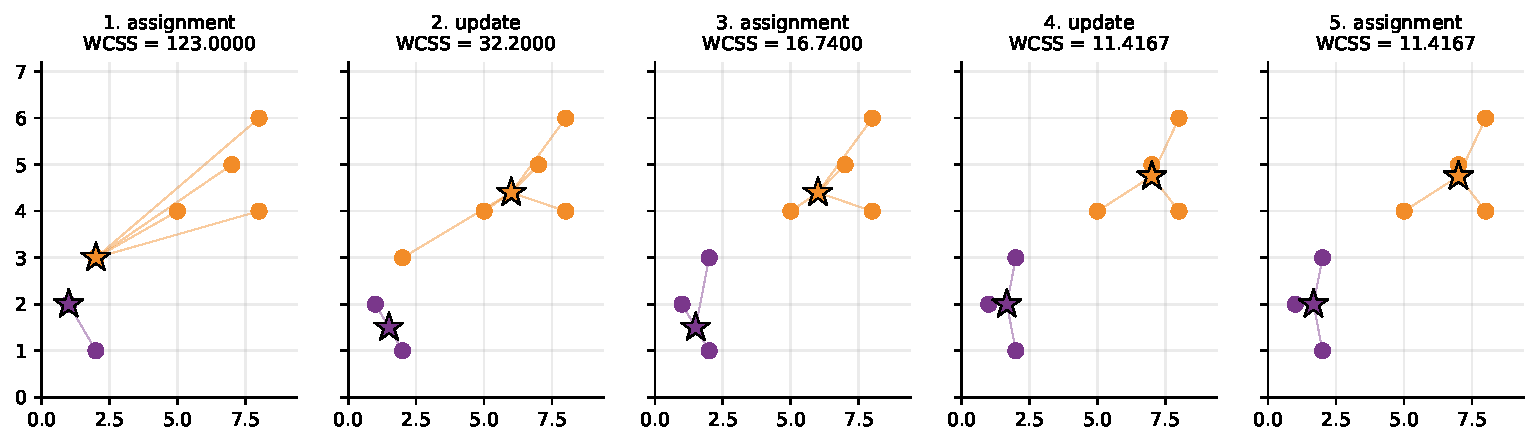
\includegraphics[width=\textwidth]{handrun.pdf}
  \end{center}
  \vspace{-0.4em}
  \begin{center}\small
    Stars are centroids; the thin lines are the distances the objective adds
    up. Panels alternate assignment, update, assignment, update, assignment
    --- and the last panel is identical to the one before it, which is what
    ``converged'' means.
  \end{center}
\end{frame}

\begin{frame}[fragile,shrink=6]{In code: the library does exactly that}
\begin{lstlisting}[basicstyle=\ttfamily\scriptsize]
km = KMeans(n_clusters=2, init=np.array([P7[0], P7[2]]),
            n_init=1, algorithm="lloyd").fit(P7)
print(km.labels_, km.cluster_centers_, km.inertia_, km.n_iter_)
\end{lstlisting}
\begin{outblk}
sklearn labels    [0 0 0 1 1 1 1]        hand labels  [0 0 0 1 1 1 1]
sklearn centres   [[1.6667, 2.0], [7.0, 4.75]]
hand centres      [[1.6667, 2.0], [7.0, 4.75]]
sklearn inertia_ 11.416667    hand WCSS 11.416667    match to 1e-12: True
iterations n_iter_ = 3
\end{outblk}
  \vspace{0.2em}
  \begin{alertblock}{And it is the global optimum here --- checked exhaustively}
    \centering\small
    All $2^{6}-1 = 63$ two-way partitions of seven points were scored.
    The best is WCSS $= \mathbf{11.4167}$ with
    $\{P_1,P_2,P_3\}$ against $\{P_4,P_5,P_6,P_7\}$ --- the answer Lloyd
    found. \textbf{On seven points. Do not generalise from that.}
  \end{alertblock}
\end{frame}

% =====================================================================
\section[Convergence]{Why it converges, and to what}
\label{sec:conv}

\begin{frame}[shrink=8]{The convergence argument, in three lines}
  \begin{block}{1. The assignment step cannot increase WCSS}
    \small Each point is moved to the centroid nearest it. Its own
    contribution $\min_j \lVert x - c_j\rVert^2$ can only fall or stay. Sum
    over points.
  \end{block}
  \begin{block}{2. The update step cannot increase WCSS}
    \small For a fixed set $S$, the point minimising
    $\sum_{x \in S}\lVert x - z\rVert^2$ is $z = \bar{x}$, the mean. Setting
    $c_j$ to the mean of $C_j$ is therefore optimal for that cluster.
    \\[0.2em]
    (Proof: $\sum_{x\in S}\lVert x-z\rVert^2 =
      \sum_{x\in S}\lVert x-\bar x\rVert^2 + |S|\,\lVert \bar x - z\rVert^2$,
     and the second term is minimised at $z=\bar x$. \ensuremath{\square})
  \end{block}
  \begin{exampleblock}{3. There are finitely many assignments}
    \small $S(n,k)$ of them. A sequence that never increases and never
    repeats a strictly better value cannot run for ever. \textbf{So the
    algorithm halts.}
  \end{exampleblock}
\end{frame}

\begin{frame}[fragile,shrink=6]{Measured: the objective after every half step}
\begin{outblk}
  step              WCSS
  assign 1         123.0000
  update 1          32.2000     <-- centres move to the means
  assign 2          16.7400     <-- P3 crosses over
  update 2          11.4167     <-- centres move again
  assign 3          11.4167     <-- nothing changes: stop
  strictly non-increasing: True
\end{outblk}
  \vspace{0.2em}
  \begin{center}
    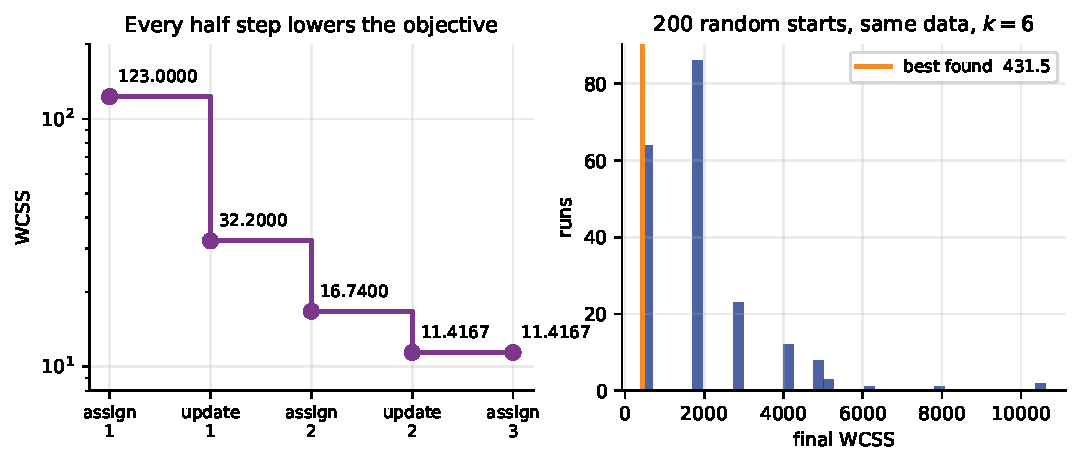
\includegraphics[width=0.86\textwidth]{wcss.pdf}
  \end{center}
\end{frame}

\begin{frame}[shrink=6]{Predict first \#3 --- how bad can a bad start be?}
  \begin{alertblock}{Commit to a number}
    Six well-separated Gaussian blobs, $600$ points, $k = 6$. Run $k$-means
    twenty times from \textbf{uniformly random} initial centroids, changing
    only the seed. The best run reaches WCSS $431.54$ and recovers the blobs
    exactly (ARI $1.000$).

    \medskip
    \centering\large
    What is the \emph{worst} of the twenty, as a multiple of the best?
  \end{alertblock}
  \onslide<2->{
  \begin{exampleblock}{}
    \centering\large
    Worst $= 5010.58$, which is $\mathbf{11.6\times}$ the best.\\
    \textbf{Twelve distinct final WCSS values} out of twenty runs.
  \end{exampleblock}
  \begin{center}\small
    Every one of those twelve is a \emph{local} optimum: no single point can
    be reassigned and no centre moved to improve it. The algorithm did
    nothing wrong. It converged. It just converged somewhere else.
  \end{center}}
\end{frame}

\begin{frame}[fragile,shrink=8]{The twenty runs, in full}
\begin{outblk}
 seed   inertia     ARI  |  seed   inertia     ARI  |  seed   inertia     ARI
    0   431.5370  1.0000 |     7  5010.5833  0.5825 |    14  1719.5194  0.7697
    1   431.5370  1.0000 |     8  1884.4493  0.7673 |    15  2737.9794  0.7718
    2   431.5370  1.0000 |     9  1885.0220  0.7677 |    16   431.5370  1.0000
    3  2740.4734  0.7787 |    10  1720.3550  0.7697 |    17  1719.5313  0.7697
    4  1720.5136  0.7693 |    11   431.5370  1.0000 |    18   431.5370  1.0000
    5   431.5370  1.0000 |    12  1883.8297  0.7673 |    19   431.5370  1.0000
    6  2737.2417  0.7713 |    13   431.5370  1.0000 |
\end{outblk}
  \vspace{0.2em}
  \begin{columns}[T]
    \begin{column}{0.49\textwidth}
      \begin{exampleblock}{Read the ARI column}
        \small Nine runs got it perfectly right. Ten got roughly
        $0.77$ --- two true blobs merged and one split. One got $0.58$.
      \end{exampleblock}
    \end{column}
    \begin{column}{0.49\textwidth}
      \begin{alertblock}{The failure has a shape}
        \small It is always the same failure: two initial centres land in the
        same blob, so that blob is split and some other pair is merged.
        Nothing can repair it, because moving one centre across the gap makes
        WCSS worse first.
      \end{alertblock}
    \end{column}
  \end{columns}
\end{frame}

\begin{frame}[shrink=4]{Drawn: three runs on the same data}
  \begin{center}
    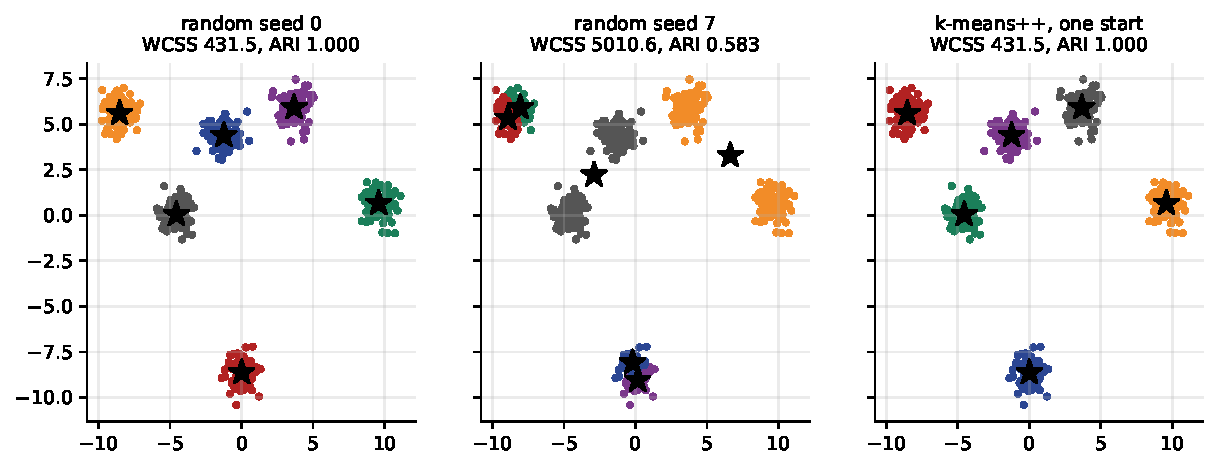
\includegraphics[width=0.98\textwidth]{seeds.pdf}
  \end{center}
  \vspace{-0.3em}
  \begin{center}\small
    Left: seed 0, the right answer. Middle: seed 7, two centres in one blob
    and three real blobs fused. Right: one $k$-means\texttt{++} start, no
    restarts, straight to the best solution.
  \end{center}
\end{frame}

\begin{frame}[fragile,shrink=8]{The fix: $k$-means\texttt{++} and \texttt{n\_init}}
  \begin{block}{$k$-means\texttt{++} seeding (Arthur and Vassilvitskii, 2007)}
    \small Pick $c_1$ uniformly at random. Then pick each further centre with
    probability proportional to $D(x)^2$, the squared distance to the nearest
    centre already chosen. Far-away points are far more likely to be picked,
    so the centres spread out. Guarantees
    $\mathbb{E}[\phi] \le 8(\ln k + 2)\,\phi_{\text{OPT}}$.
  \end{block}
\begin{outblk}
  init         mean WCSS    best      worst   % reaching best   (200 single starts)
  random      1907.6245  431.5370 10621.5284      32.0
  k-means++    437.9858  431.5370  1721.3003      99.5

  n_init =  1 (random)   : mean 1836.85   worst 10621.53   % at best  35.0
  n_init =  3 (random)   : mean  948.52   worst  2737.75   % at best  62.5
  n_init = 10 (random)   : mean  463.74   worst  1719.53   % at best  97.5
  n_init = 25 (random)   : mean  431.54   worst   431.54   % at best 100.0
  n_init =  1 (k-means++): mean  431.54   worst   431.54   % at best 100.0
\end{outblk}
\end{frame}

\begin{frame}[fragile,shrink=6]{What that costs, and what to actually do}
\begin{outblk}
  n_init =  1  0.0009 s   n_init = 10  0.0059 s   n_init = 50  0.0227 s
  (exactly 1x, 10x and 50x the starts -- the seconds are machine-dependent)
\end{outblk}
  \vspace{0.3em}
  \begin{columns}[T]
    \begin{column}{0.49\textwidth}
      \begin{exampleblock}{The practical rule}
        \small \texttt{n\_init} restarts cost \texttt{n\_init} times as much
        and you keep the run with the lowest \texttt{inertia\_}. It is the
        cheapest insurance in machine learning: $10\times$ of a
        five-millisecond fit.
      \end{exampleblock}
    \end{column}
    \begin{column}{0.49\textwidth}
      \begin{alertblock}{Read the release notes}
        \small scikit-learn's \texttt{n\_init} default became
        \texttt{"auto"}, which is \textbf{1} for \texttt{k-means++} and
        \textbf{10} for \texttt{init="random"}. If you set
        \texttt{init="random"} and also \texttt{n\_init=1}, you have opted
        into the $32\%$ row above.
      \end{alertblock}
    \end{column}
  \end{columns}
  \vspace{0.2em}
  \begin{center}\small
    \textbf{Never report a $k$-means result from a single random start},
    and always record the seed.
  \end{center}
\end{frame}

% =====================================================================
\section[Choosing $k$]{Choosing $k$}
\label{sec:k}

\begin{frame}[shrink=6]{Two heuristics, and neither is a criterion}
  \begin{columns}[T]
    \begin{column}{0.49\textwidth}
      \begin{block}{The elbow}
        \small WCSS falls monotonically with $k$ and reaches zero at
        $k = n$, so you cannot minimise it. Instead look for the $k$ where
        the \emph{rate} of improvement collapses.
        \\[0.3em]
        Two standard automations: largest perpendicular distance to the chord
        joining the ends (``kneedle''), and largest collapse in the ratio of
        successive drops.
      \end{block}
    \end{column}
    \begin{column}{0.49\textwidth}
      \begin{block}{The silhouette}
        \small For point $i$ with mean in-cluster distance $a(i)$ and mean
        distance $b(i)$ to the nearest \emph{other} cluster,
        \[
          s(i) = \frac{b(i) - a(i)}{\max(a(i), b(i))} \in [-1, 1].
        \]
        Average over all points; pick the $k$ that maximises it.
      \end{block}
    \end{column}
  \end{columns}
  \vspace{0.2em}
  \begin{alertblock}{}
    \centering\small
    The silhouette \emph{can} be maximised, which makes it feel like a
    criterion. It is not. It rewards compact well-separated clusters ---
    that is, it rewards exactly the shape $k$-means assumes.
  \end{alertblock}
\end{frame}

\begin{frame}[shrink=8]{Predict first \#4 --- how many clusters in iris?}
  \begin{alertblock}{Commit to an answer}
    Iris, $150$ flowers, four measurements, standardised. The WCSS values for
    $k = 1 \ldots 8$ are
    \[
      600.0,\ 222.4,\ 139.8,\ 114.1,\ 90.8,\ 80.0,\ 71.6,\ 62.9 .
    \]

    \medskip
    \centering\large
    What does the elbow say? What does the silhouette say? And iris has
    \emph{three} species.
  \end{alertblock}
  \onslide<2->{
  \begin{exampleblock}{}
    \centering\large
    Chord elbow: $\mathbf{k=3}$. \quad Drop-ratio elbow: $\mathbf{k=2}$.
    \quad Silhouette: $\mathbf{k=2}$ ($0.5818$). \quad Best ARI:
    $\mathbf{k=3}$ ($0.6201$).
  \end{exampleblock}
  \begin{center}\small
    \textbf{Two automations of the same heuristic disagree with each other},
    before you even bring in the silhouette.
  \end{center}}
\end{frame}

\begin{frame}[fragile,shrink=8]{The numbers behind that}
\begin{outblk}
  iris, standardised            four clean blobs
   k      WCSS   silhouette      k      WCSS       drop   silhouette
   1   600.0000   --              1   20345.30       --   --
   2   222.3617   0.5818          2    8095.80  12249.50   0.5960
   3   139.8205   0.4599          3    1880.33   6215.47   0.7668
   4   114.0925   0.3869          4     493.25   1387.08   0.7973
   5    90.8076   0.3455          5     442.57     50.68   0.7008
   6    80.0225   0.3257          6     397.59     44.98   0.5702

  summary            chord  ratio  silhouette  ARI-best  truth
  four clean blobs       3      4           4         4      4
  iris                   3      2           2         3      3
\end{outblk}
  \vspace{0.2em}
  \begin{center}\small
    On the clean blobs the drop from $1387$ to $50.7$ is unmistakable and
    three of the four rules say $4$. On iris nothing agrees with anything.
    \textbf{Two of the three iris species genuinely overlap} --- the data
    really does look like two clusters.
  \end{center}
\end{frame}

\begin{frame}[shrink=4]{Drawn: both criteria on both data sets}
  \begin{center}
    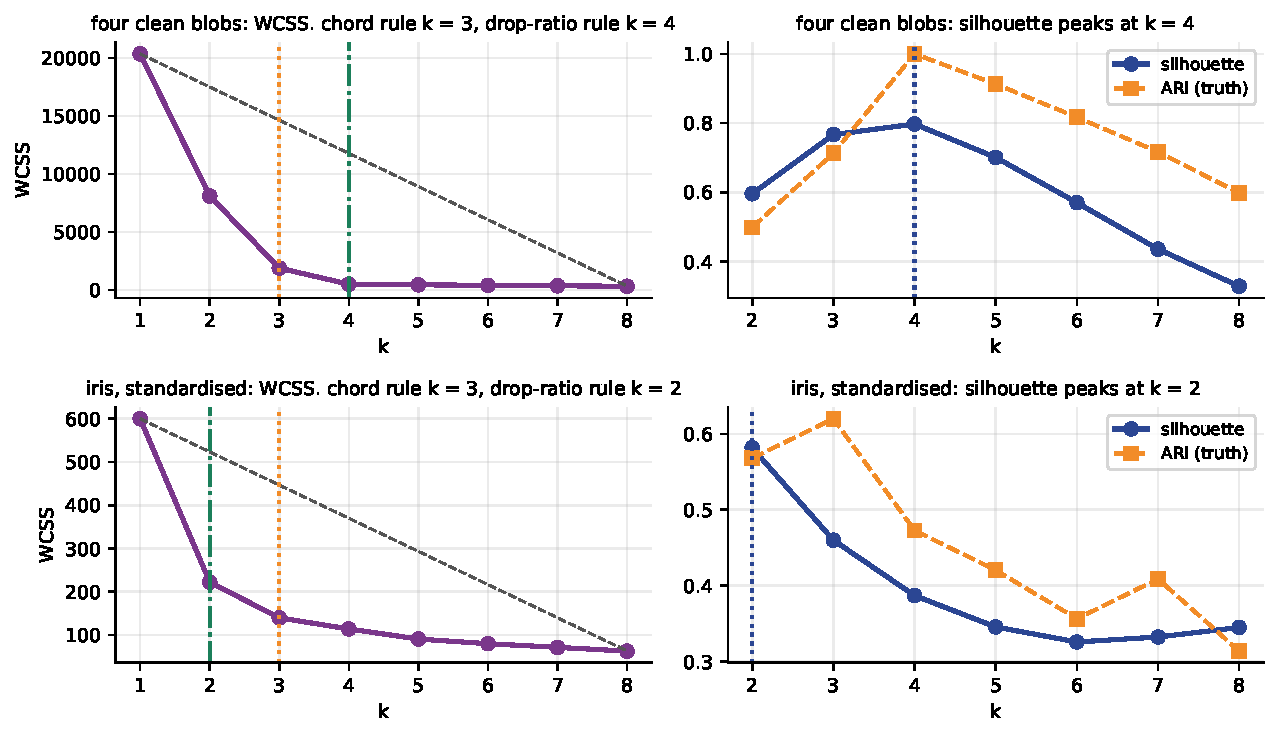
\includegraphics[width=0.86\textwidth]{choosek.pdf}
  \end{center}
  \vspace{-0.4em}
  \begin{center}\scriptsize
    Left column: WCSS with the chord (dashed grey) and the two elbow
    verdicts. Right column: silhouette against the ARI with the true labels.
  \end{center}
\end{frame}

\begin{frame}[fragile,shrink=6]{The honest version: uniform noise has an ``elbow'' too}
  \begin{center}\small
    $500$ points drawn \textbf{uniformly at random} in the unit square. There
    is no cluster structure whatsoever.
  \end{center}
\begin{outblk}
   k      WCSS   silhouette
   1    80.6344   --
   2    49.7154   0.3592
   3    31.2614   0.3839
   4    20.3558   0.4060    <-- silhouette peaks here
   5    16.6794   0.3853
   6    13.7743   0.3917
   7    11.3759   0.3895
\end{outblk}
  \vspace{0.2em}
  \begin{alertblock}{}
    \centering
    The curve is smooth, and yet the silhouette still has a maximum, at
    $k = 4$. \textbf{$k$-means always returns $k$ clusters}, whether or not
    there are any. Neither the elbow nor the silhouette will tell you the
    answer is ``none''.
  \end{alertblock}
\end{frame}

% =====================================================================
\section[Assumptions]{What $k$-means assumes, and where it breaks}
\label{sec:assume}

\begin{frame}[shrink=8]{Three assumptions hidden in one formula}
  \begin{exampleblock}{}
    \centering\large
    $\mathrm{WCSS} = \sum_j \sum_{x \in C_j} \lVert x - c_j\rVert^2$
  \end{exampleblock}
  \begin{columns}[T]
    \begin{column}{0.32\textwidth}
      \begin{block}{Spherical}
        \small A cluster is described by \emph{one point}, so the boundary
        between two clusters is the perpendicular bisector: cells of a
        Voronoi diagram, always \textbf{convex}.
      \end{block}
    \end{column}
    \begin{column}{0.32\textwidth}
      \begin{block}{Similar size}
        \small The sum is over points, so a big cluster contributes more
        terms and pulls harder. $k$-means prefers to \textbf{split a big
        cluster} rather than leave a small one alone.
      \end{block}
    \end{column}
    \begin{column}{0.32\textwidth}
      \begin{block}{Similar spread}
        \small A wide cluster and a tight one at the same distance are
        treated identically. The criterion has no notion of local density.
      \end{block}
    \end{column}
  \end{columns}
  \vspace{0.3em}
  \begin{alertblock}{}
    \centering
    These are not bugs. They are the \textbf{definition} of what $k$-means is
    looking for. If your clusters are not like that, it will still return
    $k$ of them, and they will be wrong.
  \end{alertblock}
\end{frame}

\begin{frame}[fragile,shrink=6]{Measured: four data sets it cannot handle}
\begin{outblk}
  data                    k     k-means ARI    sizes found
  two moons               2        0.274       195,205
  concentric circles      2       -0.002       207,193
  two long thin bands     2       -0.001       399,401
  very unequal sizes      3        0.288       208,176,96     (truth 400,40,40)
\end{outblk}
  \vspace{0.2em}
  \begin{columns}[T]
    \begin{column}{0.5\textwidth}
      \begin{block}{Look at the sizes}
        \small Every single answer is close to an equal split, because that
        is what minimising a sum of squares over a convex partition wants.
        On the last row the truth is $400/40/40$ and $k$-means returns
        $208/176/96$ --- \textbf{it cut the big cluster into three}.
      \end{block}
    \end{column}
    \begin{column}{0.48\textwidth}
      \begin{alertblock}{$-0.002$ and $-0.001$}
        \small An ARI at or below zero means the answer is no better than a
        random partition. On the two bands $k$-means returns a left half and
        a right half; the truth is a top band and a bottom band.
      \end{alertblock}
    \end{column}
  \end{columns}
\end{frame}

\begin{frame}[shrink=4]{Drawn: the truth, $k$-means, and (spoiler) DBSCAN}
  \begin{center}
    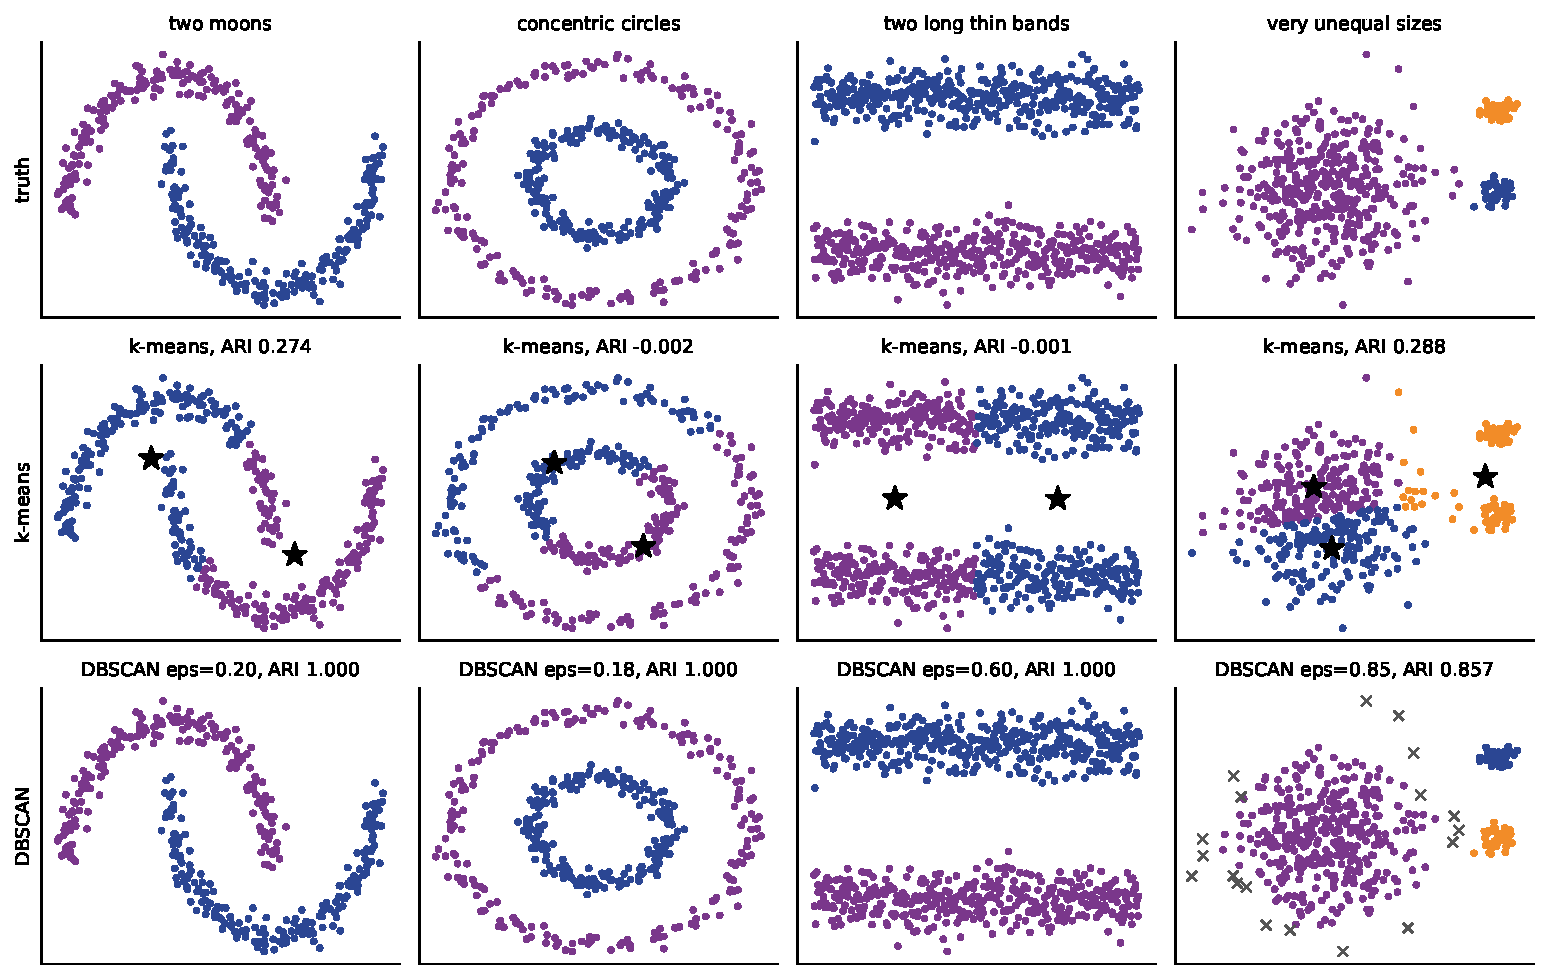
\includegraphics[width=0.80\textwidth]{assumptions.pdf}
  \end{center}
  \vspace{-0.4em}
  \begin{center}\scriptsize
    Top: the truth. Middle: $k$-means with the correct $k$, centroids
    starred. Bottom: DBSCAN --- ARI $1.000$, $1.000$, $1.000$, $0.857$ on the
    same four sets. We come back to that in the second half.
  \end{center}
\end{frame}

\begin{frame}[fragile,shrink=8]{And the mean itself is not robust}
  \begin{center}\small
    The same seven points, plus \textbf{one} extra point at $(12, 9)$.
  \end{center}
\begin{outblk}
  k-means  without the outlier: centres [[1.6667, 2.0], [7.0,  4.75]]  sizes [3, 4]
  k-means  with    the outlier: centres [[2.5,    2.5], [8.75, 6.0 ]]  sizes [4, 4]
  k-medoid without the outlier: medoids ['P1','P5'] at [[1,2],[7,5]]   E =  7.8929
  k-medoid with    the outlier: medoids ['P1','P5'] at [[1,2],[7,5]]   E = 14.2960
\end{outblk}
  \vspace{0.2em}
  \begin{columns}[T]
    \begin{column}{0.52\textwidth}
      \begin{alertblock}{One point did two things}
        \small It moved the right-hand centre by $\mathbf{2.1506}$ --- and it
        \textbf{changed the partition}: $P_4$ was dragged out of the
        right-hand cluster into the left one, giving $4/4$ instead of $3/4$.
      \end{alertblock}
    \end{column}
    \begin{column}{0.46\textwidth}
      \begin{exampleblock}{The medoid did not move}
        \small A medoid is an \emph{observation}. It cannot drift; it can
        only jump to another observation. $P_1$ and $P_5$ before, $P_1$ and
        $P_5$ after.
      \end{exampleblock}
    \end{column}
  \end{columns}
\end{frame}

\begin{frame}[fragile,shrink=6]{How far one point can move the mean}
\begin{outblk}
  outlier at    k-means: right centre      shift   sizes   k-medoids: right medoid
  none         (  7.0000,  4.7500)        0.0000   3,4     P5   (7, 5)
  (8, 6.0)     (  7.2000,  5.0000)        0.3202   3,5     P5   (7, 5)
  (10, 7.5)    (  7.6000,  5.3000)        0.8139   3,5     P5   (7, 5)
  (12, 9.0)    (  8.7500,  6.0000)        2.1506   4,4     P5   (7, 5)
  (16, 12.0)   ( 16.0000, 12.0000)       11.5569   1,7     OUT  (16, 12)
  (40, 30.0)   ( 40.0000, 30.0000)       41.5519   1,7     OUT  (40, 30)
\end{outblk}
  \vspace{0.2em}
  \begin{center}
    
\includegraphics[width=0.78\textwidth]{outlier.pdf}
  \end{center}
  \vspace{-0.3em}
  \begin{center}\scriptsize
    Beyond about $(16,12)$ \emph{both} methods give up a whole cluster to the
    single outlier --- $k$-medoids is more robust, not immune.
  \end{center}
\end{frame}

% =====================================================================
\section[$k$-medoids]{$k$-medoids and PAM}
\label{sec:medoid}

\begin{frame}[shrink=8]{Change one word in the objective}
  \begin{columns}[T]
    \begin{column}{0.48\textwidth}
      \begin{block}{$k$-means}
        \[ \sum_{j}\sum_{x\in C_j}\lVert x - c_j\rVert_2^2 \]
        \small $c_j$ is the \textbf{mean} --- a computed point, usually not
        in the data. Needs a vector space and squared Euclidean distance.
      \end{block}
    \end{column}
    \begin{column}{0.48\textwidth}
      \begin{exampleblock}{$k$-medoids}
        \[ E = \sum_{j}\sum_{x\in C_j} d(x,\ o_j) \]
        \small $o_j$ is the \textbf{medoid} --- an actual object of the data
        set. $d$ is \emph{any} dissimilarity. Not squared.
      \end{exampleblock}
    \end{column}
  \end{columns}
  \vspace{0.3em}
  \begin{block}{Three consequences, all of them the point of the method}
    \small
    \textbf{1.} The representative is a real object, so it is interpretable
    --- ``this customer is the archetype''. \\
    \textbf{2.} Any dissimilarity works: edit distance, Jaccard, Gower, a
    precomputed matrix. There is no mean of two DNA sequences; there is a
    medoid. \\
    \textbf{3.} An unsquared distance to a real point is far less sensitive
    to outliers than a squared distance to a movable mean.
  \end{block}
\end{frame}

\begin{frame}[fragile,shrink=10]{PAM: Partitioning Around Medoids}
\begin{lstlisting}[language=]
BUILD : pick the object minimising total dissimilarity to everything;
        then repeatedly add the object that reduces E the most, until k

SWAP  : repeat
            for every medoid o_i and every non-medoid o_h:
                compute the change in E if o_i were replaced by o_h
            if the best change is negative: perform that swap
            else: stop
\end{lstlisting}
  \begin{columns}[T]
    \begin{column}{0.5\textwidth}
      \begin{exampleblock}{The cost per SWAP iteration}
        \small $k(n-k)$ candidate swaps, each needing every object
        re-examined: \textbf{$O(k(n-k)^2)$} per iteration. That single
        expression is the reason CLARA exists.
      \end{exampleblock}
    \end{column}
    \begin{column}{0.48\textwidth}
      \begin{alertblock}{And $O(n^2)$ memory}
        \small PAM works from the dissimilarity matrix, exactly like
        hierarchical clustering, so it inherits the same memory wall.
      \end{alertblock}
    \end{column}
  \end{columns}
\end{frame}

\begin{frame}[fragile,shrink=8]{By hand: score all $\binom{7}{2} = 21$ medoid pairs}
  \begin{columns}[T]
    \begin{column}{0.49\textwidth}
\begin{outblk}
  {P1,P2}  E =  26.5784
  {P1,P3}  E =  22.7526
  {P1,P4}  E =  11.6700
  {P1,P5}  E =   7.8929   <-- best
  {P1,P6}  E =   9.2426
  {P1,P7}  E =   9.8482
  {P2,P3}  E =  22.7526
  {P2,P4}  E =  12.2558
  {P2,P5}  E =   8.4787
  {P2,P6}  E =   9.8284
  {P2,P7}  E =  10.4340
\end{outblk}
    \end{column}
    \begin{column}{0.49\textwidth}
\begin{outblk}
  {P3,P4}  E =  12.2558
  {P3,P5}  E =   8.4787
  {P3,P6}  E =   9.8284
  {P3,P7}  E =   9.9907
  {P4,P5}  E =  14.7055
  {P4,P6}  E =  15.2913
  {P4,P7}  E =  15.2913
  {P5,P6}  E =  22.1468
  {P5,P7}  E =  22.1468
  {P6,P7}  E =  24.4853
\end{outblk}
      \begin{exampleblock}{}
        \centering\small
        $E(\{P_1,P_5\}) = 0 + 1.4142 + 1.4142 + 2.2361 + 0 + 1.4142 + 1.4142
        = \mathbf{7.8929}$
      \end{exampleblock}
    \end{column}
  \end{columns}
  \vspace{0.2em}
  \begin{center}\small
    Twenty-one numbers is small enough to brute-force. At $n = 100$ and
    $k = 5$ it is $75{,}287{,}520$ --- which is why PAM does a local search
    instead.
  \end{center}
\end{frame}

\begin{frame}[fragile,shrink=6]{By hand: the SWAP step from a bad start}
\begin{outblk}
  start with medoids {P1, P2}, E = 26.5784
  step 1: best swap  P2 -> P5   dE = -18.6855   E =  7.8929
  step 2: best swap  P1 -> P2   dE =  +0.5858   E =  8.4787
          no swap improves E -- STOP
  final medoids: {P1, P5}   E = 7.8929
\end{outblk}
  \vspace{0.3em}
  \begin{columns}[T]
    \begin{column}{0.5\textwidth}
      \begin{block}{Reading step 2}
        \small The \emph{best} of the ten remaining candidate swaps still
        makes $E$ worse, by $0.5858$. That is the stopping condition:
        \textbf{no single swap improves the objective}, so we are at a local
        optimum of the swap neighbourhood.
      \end{block}
    \end{column}
    \begin{column}{0.48\textwidth}
      \begin{alertblock}{Same shape of guarantee as $k$-means}
        \small $E$ never increases, the number of medoid sets is finite
        $\bigl(\binom{n}{k}\bigr)$, so PAM terminates --- at a
        \textbf{local} optimum. Both methods are hill-climbers.
      \end{alertblock}
    \end{column}
  \end{columns}
\end{frame}

\begin{frame}[fragile,shrink=8]{Robustness, measured rather than asserted}
  \begin{center}\small
    Two clean blobs of $150$ points at $(0,0)$ and $(6,0)$, contaminated with
    a few points scattered in $[20,45]^2$. ``Centre error'' is the largest
    distance from a true centre to the nearest thing the method returned.
  \end{center}
\begin{outblk}
  outliers  k-means: centre error  ARI  |  k-medoids: medoid error  ARI
       0              0.0951   1.000  |                0.0905   1.000
       2              0.5210   1.000  |                0.0905   1.000
       5              3.0826   0.000  |                0.0905   1.000
      10              3.0826   0.000  |                0.0905   1.000
      20              3.0826   0.000  |                4.0563   0.000
\end{outblk}
  \vspace{0.2em}
  \begin{alertblock}{}
    \centering
    \textbf{Five} outliers out of $305$ points destroy $k$-means: it spends a
    centre on them and merges the two real clusters, ARI $1.000 \to 0.000$.
    Two are already enough to drag a centre five times further off.
    $k$-medoids does not move until there are $20$. \textbf{Robust, not
    immune.}
  \end{alertblock}
\end{frame}

\begin{frame}[fragile,shrink=6]{And it runs where $k$-means cannot run at all}
  \begin{center}\small
    Eight words, Levenshtein edit distance, $k = 2$. There is no arithmetic
    mean of two words, so $k$-means is simply not defined here.
  \end{center}
\begin{outblk}
  medoids: ['cluster', 'density']   E = 19.0
  cluster 1: cluster, clusters, clustered
  cluster 2: medoid, medoids, density, densities, dense
\end{outblk}
  \vspace{0.3em}
\begin{outblk}
     n    k   PAM time (s)   k-means time (s)    ratio
   250    4        0.0016            0.0037           0.4x
   500    4        0.0100            0.0049           2.1x
  1000    4        0.0378            0.0054           7.0x
  2000    4        0.1817            0.0066          27.6x
  4000    4        1.1032            0.0073         150.3x
  fitted exponent for PAM,  t = c n^p :  p = 2.30
  exact: PAM needs n(n-1)/2 = 7,998,000 distances before its first swap;
         k-means needs n*k = 16,000 per iteration.  A factor of 500.
\end{outblk}
  \vspace{0.1em}
  \begin{center}\small
    Faster than $k$-means at $n = 250$; two orders of magnitude slower at
    $n = 4000$, growing like $n^{2.3}$. Quote the count, not the clock:
    \textbf{$500\times$ the distances} before the first swap.
  \end{center}
\end{frame}

% =====================================================================
\section[CLARA]{CLARA: Clustering Large Applications}
\label{sec:clara}

\begin{frame}{Predict first \#5 --- PAM on a hundred thousand rows}
  \begin{alertblock}{Commit to two numbers}
    You have $100{,}000$ records and you want $k = 5$ medoids.

    \medskip
    \centering\large
    How many candidate swaps does \emph{one} SWAP iteration consider?
    And how big is the dissimilarity matrix PAM needs?
  \end{alertblock}
  \onslide<2->{
  \begin{exampleblock}{}
    \centering\large
    $k(n-k)^2 = 5 \times 99995^2 = \mathbf{5.0 \times 10^{10}}$
    evaluations per iteration.\\[0.3em]
    The $n \times n$ float64 matrix is $\mathbf{74.5\ \text{GiB}}$.
  \end{exampleblock}
  \begin{center}\small
    And PAM does not run for one iteration. \textbf{Both numbers have to
    come down, and the only lever available is $n$.}
  \end{center}}
\end{frame}

\begin{frame}[fragile,shrink=8]{CLARA, in six lines}
\begin{lstlisting}[language=]
Input : n objects, k, a sample size s (Kaufman and Rousseeuw suggest 40 + 2k)
best = None
repeat 5 times:
    S    = a random sample of s objects from the data
    M    = PAM(S, k)                      # only s x s dissimilarities needed
    cost = sum over ALL n objects of d(object, nearest medoid in M)
    if cost < best.cost: best = (M, cost)
return best
\end{lstlisting}
  \begin{columns}[T]
    \begin{column}{0.52\textwidth}
      \begin{exampleblock}{The complexity, and why it works}
        \small $O(k s^2 + k(n-k))$ per sample, so \textbf{linear in $n$}, and
        the matrix is $s \times s$, not $n \times n$. The evaluation step
        touches all $n$ objects, which is what stops a lucky sample from
        looking better than it is.
      \end{exampleblock}
    \end{column}
    \begin{column}{0.46\textwidth}
      \begin{alertblock}{Two honest limitations}
        \small \textbf{1.} CLARA can only return medoids that appeared in one
        of its samples. \textbf{2.} It is randomised, so two runs give two
        answers.
      \end{alertblock}
    \end{column}
  \end{columns}
\end{frame}

\begin{frame}[fragile,shrink=6]{Measured: PAM against CLARA on the same data}
\begin{outblk}
      n    PAM time   PAM cost    CLARA time  CLARA cost   cost ratio   speed-up
    500       0.012    661.537       0.002    707.320      1.0692        5.2x
   1000       0.033   1290.963       0.003   1342.576      1.0400       12.4x
   2000       0.268   2636.569       0.004   2842.923      1.0783       66.1x
   4000       1.731   5261.167       0.004   5490.189      1.0435      421.0x
\end{outblk}
  \vspace{0.2em}
  \begin{center}
    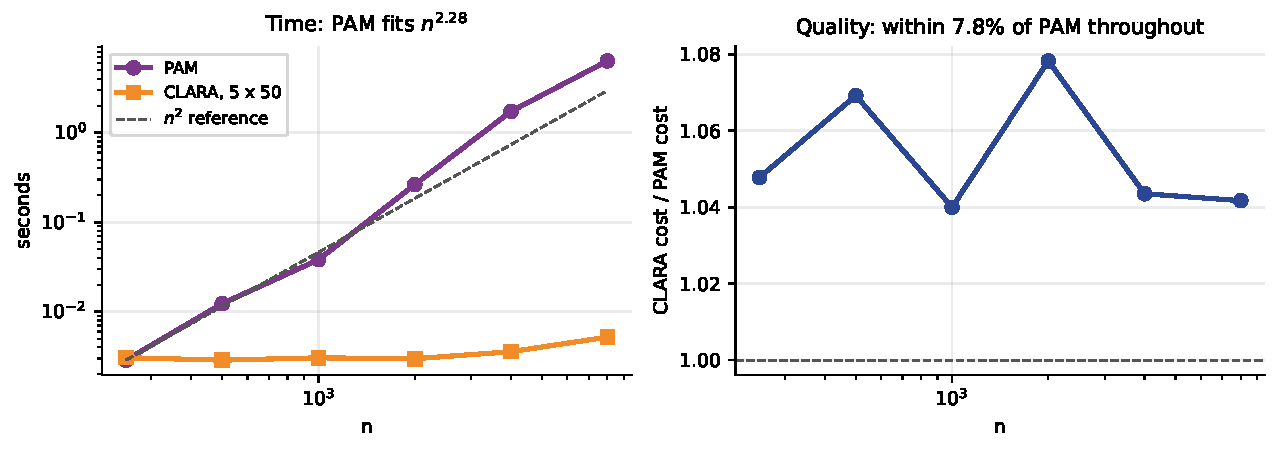
\includegraphics[width=0.78\textwidth]{clara.pdf}
  \end{center}
  \vspace{-0.3em}
  \begin{center}\scriptsize
    CLARA's time barely moves, because the PAM it runs is always on $50$
    objects. Only the final assignment sweep grows with $n$.
  \end{center}
\end{frame}

\begin{frame}[fragile,shrink=8]{The trade, in two tables}
\begin{outblk}
  n = 4000, k = 5.  PAM reference: cost 5261.167   ARI 0.8404
  sample size   samples   CLARA cost   cost/PAM     ARI    time (s)
           20         5     5915.642     1.1244  0.8008     0.003
           50         5     5490.189     1.0435  0.8266     0.004
          250         5     5319.240     1.0110  0.8384     0.015
          500         5     5302.009     1.0078  0.8302     0.048

  CLARA over 10 seeds: cost 5421.410 to 5708.138 (spread 5.3%),
                       ARI 0.8052 to 0.8290.   PAM is deterministic.
\end{outblk}
  \vspace{0.2em}
  \begin{columns}[T]
    \begin{column}{0.5\textwidth}
      \begin{exampleblock}{Buy quality with sample size}
        \small $s = 20$ costs $12\%$ more than PAM; $s = 500$ costs
        $0.8\%$ more and is still far faster than PAM at this $n$.
      \end{exampleblock}
    \end{column}
    \begin{column}{0.48\textwidth}
      \begin{alertblock}{Say this out loud in the lab}
        \small CLARA gives a \textbf{different answer on every seed}. Report
        the seed, or run several and keep the best cost --- which is what
        CLARA is already doing internally, five times.
      \end{alertblock}
    \end{column}
  \end{columns}
\end{frame}

\begin{frame}[fragile,shrink=8]{One thing CLARA is \emph{not} guilty of}
  \begin{center}\small
    $6040$ points: two clusters of $3000$ and one of $40$. A sample of $50$
    contains, on average, $0.33$ points from the small cluster.
  \end{center}
\begin{outblk}
  PAM   medoids at [[9.44, 0.43], [10.62, -0.51], [0.04, 0.02]]  cost 7239.719
  cost if a medoid is forced onto each true centre:              7502.069
  CLARA sample   50  cost 7269.834  ratio 1.0042  ARI 0.7426
  CLARA sample 1000  cost 7254.729  ratio 1.0021  ARI 0.7457
\end{outblk}
  \vspace{0.3em}
  \begin{alertblock}{Read the second line}
    \centering
    \textbf{PAM itself puts two medoids in one big cluster and none on the
    $40$}, and the ``correct'' solution is genuinely more expensive:
    $7502$ against $7240$. So this is a property of the \textbf{objective},
    not of the sampling. \emph{Minimising total dissimilarity does not
    reward small clusters.}
  \end{alertblock}
\end{frame}

% =====================================================================
\section[DBSCAN]{Density-based clustering: DBSCAN}
\label{sec:dbscan}

\begin{frame}[shrink=6]{A completely different definition of ``cluster''}
  \begin{columns}[T]
    \begin{column}{0.48\textwidth}
      \begin{block}{Partitioning says}
        A cluster is \textbf{the set of points nearest to a representative}.
        Consequences: convex, you must supply $k$, every point is in a
        cluster.
      \end{block}
    \end{column}
    \begin{column}{0.48\textwidth}
      \begin{exampleblock}{Density says}
        A cluster is \textbf{a connected region where the points are packed
        closely together}, separated from other such regions by sparse
        space. Consequences: any shape, $k$ discovered, and points in the
        sparse space belong to \textbf{nothing}.
      \end{exampleblock}
    \end{column}
  \end{columns}
  \vspace{0.4em}
  \begin{alertblock}{}
    \centering
    \textbf{DBSCAN} --- Density-Based Spatial Clustering of Applications with
    Noise, Ester, Kriegel, Sander and Xu, KDD 1996. Two parameters, no $k$,
    and an explicit category for ``this point is not in any cluster''.
  \end{alertblock}
\end{frame}

\begin{frame}[shrink=12]{The definitions, precisely}
  \begin{block}{Two parameters}
    \small $\varepsilon$ (\texttt{eps}), a radius; and \emph{minPts}
    (\texttt{min\_samples}), a count. The
    \textbf{$\varepsilon$-neighbourhood} of $p$ is
    $N_\varepsilon(p) = \{q : d(p,q) \le \varepsilon\}$, \emph{including $p$
    itself} in scikit-learn's convention.
  \end{block}
  \begin{columns}[T]
    \begin{column}{0.33\textwidth}
      \begin{exampleblock}{Core}
        \small $|N_\varepsilon(p)| \ge$ minPts. The point sits in a dense
        region.
      \end{exampleblock}
    \end{column}
    \begin{column}{0.33\textwidth}
      \begin{exampleblock}{Border}
        \small Not core, but lies inside $N_\varepsilon(q)$ for some
        \emph{core} $q$. On the edge of a dense region.
      \end{exampleblock}
    \end{column}
    \begin{column}{0.33\textwidth}
      \begin{exampleblock}{Noise}
        \small Neither. Belongs to no cluster and is reported as
        \texttt{-1}.
      \end{exampleblock}
    \end{column}
  \end{columns}
  \vspace{0.3em}
  \begin{block}{Density-reachability, which is what glues a cluster together}
    \small
    $q$ is \textbf{directly density-reachable} from a core point $p$ if
    $q \in N_\varepsilon(p)$. \quad
    $q$ is \textbf{density-reachable} from $p$ if there is a chain
    $p = p_1, \ldots, p_m = q$ with each $p_{i+1}$ directly
    density-reachable from $p_i$ (so $p_1 \ldots p_{m-1}$ are all core).
    \quad Two points are \textbf{density-connected} if both are
    density-reachable from a common core point. \textbf{A cluster is a
    maximal density-connected set.}
  \end{block}
\end{frame}

\begin{frame}[fragile,shrink=6]{Eleven points, $\varepsilon = 1.5$, minPts $= 3$}
  \begin{center}\small
    $Q_1(1,1)\ Q_2(2,1)\ Q_3(1,2)\ Q_4(2,2)\ Q_5(3,3)\ Q_6(7,3)\ Q_7(8,3)\
     Q_8(8,4)\ Q_9(9,5)\ Q_{10}(5,6)\ Q_{11}(11,1)$
  \end{center}
\begin{outblk}
          Q1     Q2     Q3     Q4     Q5     Q6     Q7     Q8     Q9    Q10    Q11
  Q1   0.000  1.000  1.000  1.414  2.828  6.325  7.280  7.616  8.944  6.403 10.000
  Q2   1.000  0.000  1.414  1.000  2.236  5.385  6.325  6.708  8.062  5.831  9.000
  Q3   1.000  1.414  0.000  1.000  2.236  6.083  7.071  7.280  8.544  5.657 10.050
  Q4   1.414  1.000  1.000  0.000  1.414  5.099  6.083  6.325  7.616  5.000  9.055
  Q5   2.828  2.236  2.236  1.414  0.000  4.000  5.000  5.099  6.325  3.606  8.246
  Q6   6.325  5.385  6.083  5.099  4.000  0.000  1.000  1.414  2.828  3.606  4.472
  Q7   7.280  6.325  7.071  6.083  5.000  1.000  0.000  1.000  2.236  4.243  3.606
  Q8   7.616  6.708  7.280  6.325  5.099  1.414  1.000  0.000  1.414  3.606  4.243
  Q9   8.944  8.062  8.544  7.616  6.325  2.828  2.236  1.414  0.000  4.123  4.472
  Q10  6.403  5.831  5.657  5.000  3.606  3.606  4.243  3.606  4.123  0.000  7.810
  Q11 10.000  9.000 10.050  9.055  8.246  4.472  3.606  4.243  4.472  7.810  0.000
\end{outblk}
  \vspace{0.1em}
  \begin{center}\scriptsize
    Only two values matter against $\varepsilon = 1.5$: $1.000$ and
    $\sqrt{2} = 1.414$ are in; $2.000$ and $\sqrt{5} = 2.236$ are out.
  \end{center}
\end{frame}

\begin{frame}[shrink=8]{Predict first \#6 --- classify three of them}
  \begin{alertblock}{Commit to three answers}
    $\varepsilon = 1.5$, minPts $= 3$, counting the point itself.

    \medskip
    \centering\large
    Is $Q_5(3,3)$ core, border or noise? \\
    Is $Q_9(9,5)$? \\
    Is $Q_{10}(5,6)$?
  \end{alertblock}
  \onslide<2->{
  \begin{exampleblock}{}
    \centering
    $N_\varepsilon(Q_5) = \{Q_5, Q_4\}$, size $2 < 3$: \textbf{not core}. But
    $Q_5 \in N_\varepsilon(Q_4)$ and $Q_4$ is core, so $Q_5$ is
    \textbf{BORDER}.\\[0.2em]
    $N_\varepsilon(Q_9) = \{Q_9, Q_8\}$, size $2$; $Q_8$ is core, so $Q_9$ is
    \textbf{BORDER}.\\[0.2em]
    $N_\varepsilon(Q_{10}) = \{Q_{10}\}$, size $1$, and it is in nobody
    else's ball: \textbf{NOISE}.
  \end{exampleblock}
  \begin{center}\small
    The commonest mistake is forgetting the point counts itself. With
    minPts $= 3$ a core point needs \textbf{two} other points within
    $\varepsilon$, not three.
  \end{center}}
\end{frame}

\begin{frame}[fragile,shrink=8]{By hand: every point, arithmetically}
\begin{outblk}
  point   coord     N_eps(p)                       |N|  verdict
  Q1     ( 1, 1)  {Q1,Q2,Q3,Q4                 }   4  CORE
  Q2     ( 2, 1)  {Q1,Q2,Q3,Q4                 }   4  CORE
  Q3     ( 1, 2)  {Q1,Q2,Q3,Q4                 }   4  CORE
  Q4     ( 2, 2)  {Q1,Q2,Q3,Q4,Q5              }   5  CORE
  Q5     ( 3, 3)  {Q4,Q5                       }   2  BORDER
  Q6     ( 7, 3)  {Q6,Q7,Q8                    }   3  CORE
  Q7     ( 8, 3)  {Q6,Q7,Q8                    }   3  CORE
  Q8     ( 8, 4)  {Q6,Q7,Q8,Q9                 }   4  CORE
  Q9     ( 9, 5)  {Q8,Q9                       }   2  BORDER
  Q10    ( 5, 6)  {Q10                         }   1  NOISE
  Q11    (11, 1)  {Q11                         }   1  NOISE
  core 7, border 2, noise 2
\end{outblk}
  \vspace{0.1em}
  \begin{center}\small
    $Q_6$ and $Q_7$ each have exactly $3$: \textbf{core by one point}. Change
    minPts to $4$ and the right-hand cluster loses its core.
  \end{center}
\end{frame}

\begin{frame}[fragile,shrink=6]{By hand: chain the core points into clusters}
\begin{outblk}
  cluster 1 grown from Q1: core points {Q1,Q2,Q3,Q4}, then border Q5 joins
  cluster 2 grown from Q6: core points {Q6,Q7,Q8}, then border Q9 joins
  cluster 1 = {Q1,Q2,Q3,Q4,Q5}
  cluster 2 = {Q6,Q7,Q8,Q9}
  noise     = {Q10,Q11}
\end{outblk}
  \vspace{0.3em}
  \begin{columns}[T]
    \begin{column}{0.52\textwidth}
      \begin{block}{The procedure, exactly}
        \small Take any unvisited core point, take everything
        density-reachable from it --- that is one cluster. Repeat. Whatever
        is left over is noise. Border points are attached to \textbf{whichever
        core cluster reached them first}.
      \end{block}
    \end{column}
    \begin{column}{0.46\textwidth}
      \begin{alertblock}{The one non-determinism in DBSCAN}
        \small A border point within $\varepsilon$ of two different clusters
        is assigned by visiting order. Core points and noise are never
        ambiguous. Here no border point is contested.
      \end{alertblock}
    \end{column}
  \end{columns}
\end{frame}

\begin{frame}[shrink=10]{Drawn: the eleven points with their $\varepsilon$-balls}
  \begin{center}
    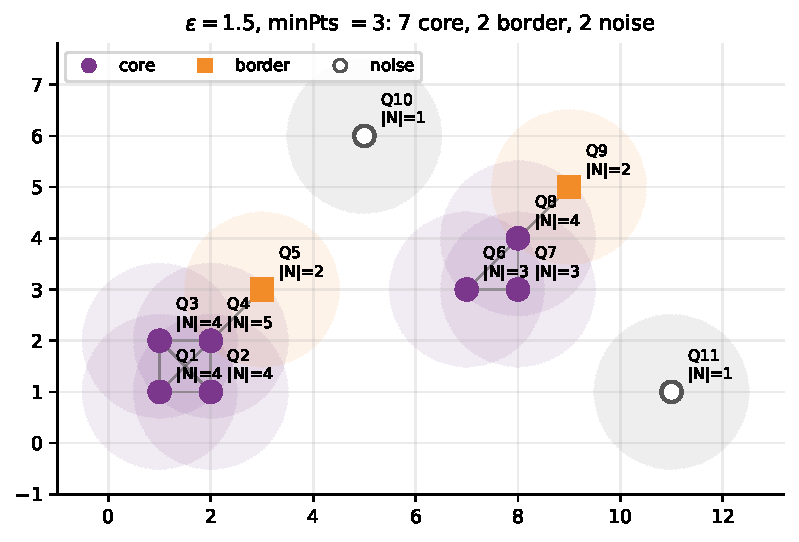
\includegraphics[width=0.66\textwidth]{dbscanhand.pdf}
  \end{center}
  \vspace{-0.3em}
  \begin{center}\small
    Circles are the $\varepsilon$-balls; grey edges join pairs within
    $\varepsilon$. Squares are border points, hollow circles are noise. Note
    that $Q_{10}$ is not far from the data --- it is $3.606$ from both
    clusters --- but $\varepsilon = 1.5$ and that is all that matters.
  \end{center}
\end{frame}

\begin{frame}[fragile,shrink=6]{In code: the library agrees exactly}
\begin{lstlisting}[basicstyle=\ttfamily\scriptsize]
db = DBSCAN(eps=1.5, min_samples=3).fit(P11)
print(db.labels_, sorted(db.core_sample_indices_))
\end{lstlisting}
\begin{outblk}
sklearn labels_       [ 0  0  0  0  0  1  1  1  1 -1 -1]
hand labels           [ 0  0  0  0  0  1  1  1  1 -1 -1]
agree (up to renaming): True
sklearn core points   ['Q1','Q2','Q3','Q4','Q6','Q7','Q8']
hand core points      ['Q1','Q2','Q3','Q4','Q6','Q7','Q8']
identical: True
\end{outblk}
  \vspace{0.3em}
  \begin{alertblock}{Two conventions worth writing down}
    \centering\small
    \texttt{labels\_} uses \textbf{$-1$ for noise} --- it is not a cluster
    index, and \texttt{np.bincount} on it will fail. \\
    \texttt{min\_samples} \textbf{counts the point itself}.
  \end{alertblock}
\end{frame}

\begin{frame}[fragile,shrink=8]{Both parameters change the answer}
\begin{outblk}
  min_samples = 2  ->  2 clusters, 2 noise, labels [0,0,0,0,0,1,1,1,1,-1,-1]
  min_samples = 3  ->  2 clusters, 2 noise, labels [0,0,0,0,0,1,1,1,1,-1,-1]
  min_samples = 4  ->  2 clusters, 2 noise, labels [0,0,0,0,0,1,1,1,1,-1,-1]
  min_samples = 5  ->  1 clusters, 6 noise, labels [0,0,0,0,0,-1,-1,-1,-1,-1,-1]

  eps = 1.0  ->  2 clusters, 4 noise, labels [0,0,0,0,-1,1,1,1,-1,-1,-1]
  eps = 1.4  ->  2 clusters, 4 noise, labels [0,0,0,0,-1,1,1,1,-1,-1,-1]
  eps = 1.5  ->  2 clusters, 2 noise, labels [0,0,0,0,0,1,1,1,1,-1,-1]
  eps = 2.5  ->  2 clusters, 2 noise, labels [0,0,0,0,0,1,1,1,1,-1,-1]
  eps = 4.5  ->  1 clusters, 0 noise, labels [0,0,0,0,0,0,0,0,0,0,0]
\end{outblk}
  \vspace{0.2em}
  \begin{center}\small
    Going from $\varepsilon = 1.4$ to $1.5$ crosses $\sqrt{2}$ and turns two
    noise points into border points. Going from minPts $3$ to $4$ destroys
    the right-hand cluster, whose core points had exactly three neighbours.
    \textbf{Both parameters are cliffs, not dials.}
  \end{center}
\end{frame}

\begin{frame}[fragile,shrink=8]{What DBSCAN buys you: shape, $k$, and noise}
\begin{outblk}
  data                    eps  minPts   ARI    clusters  noise    (k-means ARI)
  two moons              0.20     5     1.000      2        0        0.274
  concentric circles     0.18     5     1.000      2        0       -0.002
  two long thin bands    0.60     5     1.000      2        0       -0.001
  very unequal sizes     0.85     5     0.857      3       19        0.288

  blobs on a circle, eps = 0.45 and minPts = 5 held FIXED throughout:
  true k = 2  -> DBSCAN found 2   ARI 0.9265   noise  9
  true k = 3  -> DBSCAN found 3   ARI 0.9537   noise 11
  true k = 5  -> DBSCAN found 5   ARI 0.9611   noise 18
  true k = 8  -> DBSCAN found 8   ARI 0.9667   noise 26
\end{outblk}
  \vspace{0.2em}
  \begin{exampleblock}{}
    \centering
    ARI $1.000$ on three shapes where $k$-means scores $0.27$, $-0.00$ and
    $-0.00$ --- and \textbf{$k$ was never supplied}. $k$-means would have
    needed it told four times in the second block.
  \end{exampleblock}
\end{frame}

\begin{frame}[fragile,shrink=8]{And it says ``I do not know'' --- which $k$-means cannot}
  \begin{center}\small
    Three clean blobs of $300$ points, plus $60$ points scattered uniformly
    over the whole plot. $\varepsilon = 0.55$, minPts $= 5$.
  \end{center}
\begin{outblk}
  planted noise points: 60   DBSCAN called 57 points noise
  of the planted noise, correctly flagged: 55 (91.7%)
  of the genuine points, wrongly flagged:   2 ( 0.7%)
  ARI on the 300 real points: DBSCAN 0.9901   k-means 1.0000
\end{outblk}
  \vspace{0.2em}
  \begin{columns}[T]
    \begin{column}{0.49\textwidth}
      \begin{exampleblock}{}
        \small $92\%$ of the contamination identified, at the cost of two
        real points out of $300$. That column of $-1$s is a deliverable ---
        outlier detection for free.
      \end{exampleblock}
    \end{column}
    \begin{column}{0.49\textwidth}
      \begin{alertblock}{Read the ARI honestly}
        \small $k$-means scored \emph{better} on the real points here, and it
        put every one of the $60$ noise points inside a cluster. It has no
        vocabulary for ``this belongs to nothing''.
      \end{alertblock}
    \end{column}
  \end{columns}
\end{frame}

% =====================================================================
\section[One global eps]{DBSCAN's weakness: one global $\varepsilon$}
\label{sec:eps}

\begin{frame}{Predict first \#7 --- two densities, one radius}
  \begin{alertblock}{Commit to an answer}
    Three clusters of $150$ points. Two are \textbf{tight} (sd $0.12$) and
    their centres are only $1.0$ apart. The third is \textbf{loose}
    (sd $1.60$) and sits well away from both.

    \medskip
    \centering\large
    Is there a value of $\varepsilon$ that recovers all three?
  \end{alertblock}
  \onslide<2->{
  \begin{exampleblock}{}
    \centering\large
    \textbf{No.} At $\varepsilon \le 0.15$ the two tight clusters are
    perfect and \textbf{all $150$} points of the loose one are noise.
    By the time $\varepsilon$ is large enough for the loose one to appear,
    the two tight ones have been \textbf{welded into a single cluster}.
  \end{exampleblock}
  \begin{center}\small
    $\varepsilon$ is a \emph{global} density threshold. One number cannot
    describe two densities. This is the honest, examinable weakness of
    DBSCAN.
  \end{center}}
\end{frame}

\begin{frame}[fragile,shrink=8]{Measured: the whole sweep}
\begin{outblk}
   eps  clusters  noise |  tight A            tight B            loose C
  0.06       2     183 |  20 noise, 1 part   13 noise, 1 part  150 noise, 0 parts
  0.10       2     158 |   4 noise, 1 part    4 noise, 1 part  150 noise, 0 parts
  0.15       2     152 |   0 noise, 1 part    2 noise, 1 part  150 noise, 0 parts
  0.25       6     127 |   0 noise, 1 part    0 noise, 2 parts 127 noise, 4 parts  WELDED
  0.35       9      81 |   0 noise, 1 part    0 noise, 1 part   81 noise, 8 parts  WELDED
  0.50       4      54 |   0 noise, 1 part    0 noise, 1 part   54 noise, 3 parts  WELDED
  0.80       2      18 |   0 noise, 1 part    0 noise, 1 part   18 noise, 1 part   WELDED
  1.20       1       3 |   0 noise, 1 part    0 noise, 1 part    3 noise, 1 part   WELDED
\end{outblk}
  \vspace{0.2em}
  \begin{center}\small
    ``WELDED'' means the two tight clusters have been merged into one.
    Between $0.15$ and $0.25$ the loose cluster is still $85\%$ noise and the
    tight pair has already fused. \textbf{There is no window.}
    \\[0.2em]
    And $k$-means with $k = 3$ scores ARI $\mathbf{0.3937}$ on the same data
    --- it splits the loose cluster and merges the tight pair. Neither method
    is the answer here; \textbf{OPTICS and HDBSCAN exist for exactly this}.
  \end{center}
\end{frame}

\begin{frame}[shrink=4]{Drawn: the same failure}
  \begin{center}
    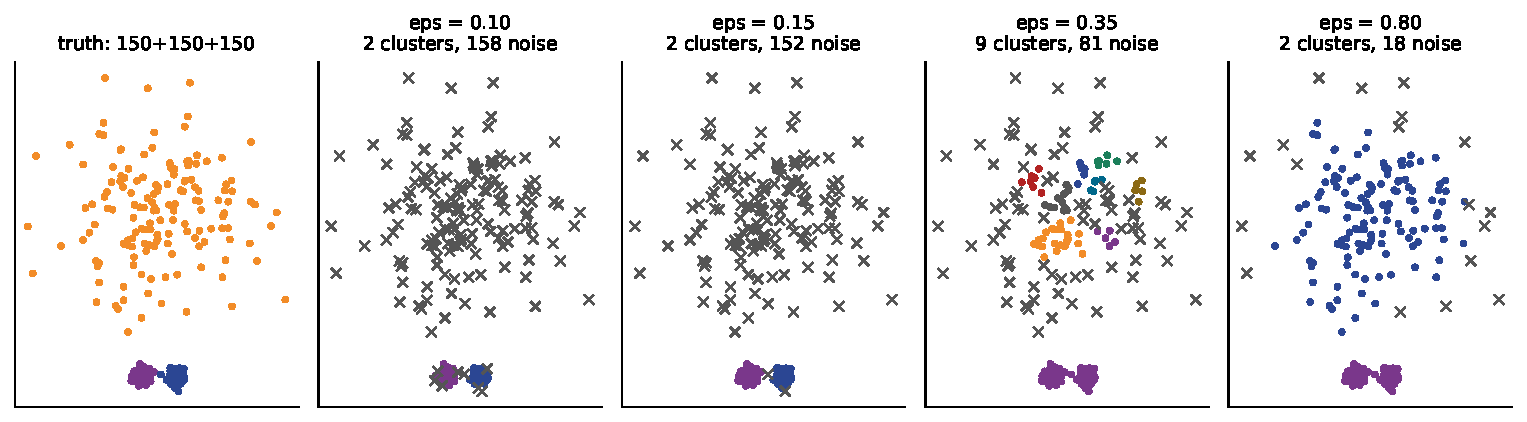
\includegraphics[width=\textwidth]{density.pdf}
  \end{center}
  \vspace{-0.4em}
  \begin{center}\scriptsize
    Grey crosses are noise. Left to right: the truth, then
    $\varepsilon = 0.10,\ 0.15,\ 0.35,\ 0.80$. Watch the top cluster appear
    only after the bottom two have merged.
  \end{center}
\end{frame}

\begin{frame}[fragile,shrink=8]{Choosing $\varepsilon$: the $k$-distance graph}
  \begin{block}{The standard recipe (Ester et al., \S4.2)}
    \small Fix minPts. For every point compute the distance to its
    $(\text{minPts}-1)$-th nearest neighbour. Sort those $n$ numbers and plot
    them. Points in a cluster have small values; noise points have large
    ones, so the curve has a \textbf{knee}. Read $\varepsilon$ off the knee.
  \end{block}
\begin{outblk}
  sorted 5th-nearest-neighbour distances, two moons, n = 400:
    10% 0.0445   25% 0.0527   50% 0.0642   75% 0.0837
    90% 0.1051   95% 0.1179   99% 0.1489  100% 0.1665
  automatic chord knee: 0.0875
\end{outblk}
  \vspace{0.2em}
  \begin{alertblock}{}
    \centering\small
    The original paper says plainly that finding the knee automatically is
    ``very difficult'' and proposes an \textbf{interactive} procedure. Our
    automatic knee gives $0.0875$ --- and that is the wrong answer, as the
    next slide shows.
  \end{alertblock}
\end{frame}

\begin{frame}[fragile,shrink=8]{What each candidate $\varepsilon$ actually gives}
\begin{outblk}
   eps   clusters  noise    ARI
  0.060     31       121    0.031
  0.080     13        41    0.185
  0.087      7        24    0.320   <-- the automatic knee
  0.100      4        10    0.731
  0.105      4         5    0.744   <-- 90th percentile
  0.118      3         2    0.921   <-- 95th percentile
  0.150      2         0    1.000
  0.200      2         0    1.000
  0.250      2         0    1.000
  0.270      1         0    0.000
  0.300      1         0    0.000
\end{outblk}
  \vspace{0.2em}
  \begin{center}
    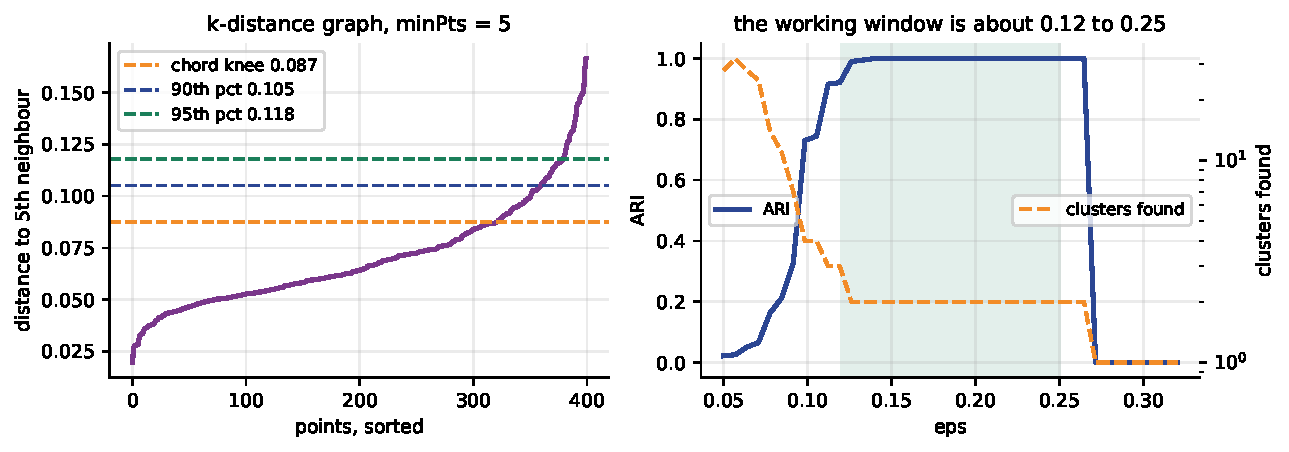
\includegraphics[width=0.68\textwidth]{kdist.pdf}
  \end{center}
\end{frame}

\begin{frame}[shrink=8]{So how sensitive is it, exactly?}
  \begin{columns}[T]
    \begin{column}{0.5\textwidth}
      \begin{alertblock}{The working window is a factor of two}
        \small $0.12$ to $0.25$ gives ARI $\approx 1$. Just below it,
        $0.08$ gives \textbf{13 clusters}. Just above it, $0.27$ gives
        \textbf{1 cluster}. Between $0.25$ and $0.27$ the answer collapses
        completely.
      \end{alertblock}
    \end{column}
    \begin{column}{0.48\textwidth}
      \begin{block}{What the graph is actually for}
        \small It converts ``pick a positive real number'' into ``pick
        something between about $0.09$ and $0.17$'' and then you look at the
        result. \textbf{It narrows the search. It does not end it.}
      \end{block}
    \end{column}
  \end{columns}
  \vspace{0.3em}
  \begin{exampleblock}{Rules of thumb worth remembering}
    \small
    minPts $\ge d+1$, commonly $2d$; Ester et al.\ used $4$ for
    two-dimensional data. Larger minPts means more noise and more robustness.
    \textbf{Scale your features first} --- $\varepsilon$ is a distance, so
    one column in rupees and one in metres makes it meaningless.
  \end{exampleblock}
\end{frame}

\begin{frame}[fragile,shrink=8]{And in high dimensions, $\varepsilon$ stops meaning anything}
\begin{outblk}
  d      median 5-NN distance   ratio max/min NN distance
    2            0.1742              300.4036
    5            1.0580                9.6541
   10            2.3147                3.2597
   20            4.1659                2.4595
   50            7.8523                1.6474
  100           12.0239                1.3444
\end{outblk}
  \vspace{0.2em}
  \begin{columns}[T]
    \begin{column}{0.52\textwidth}
      \begin{block}{Read the right-hand column}
        \small In two dimensions the loneliest point is $300\times$ further
        from its neighbour than the most crowded one. At $d = 100$ that ratio
        is $1.34$: \textbf{every point is about equally far from every other
        point}, so no threshold separates dense from sparse.
      \end{block}
    \end{column}
    \begin{column}{0.46\textwidth}
      \begin{alertblock}{Measured on real data}
        \small With $\varepsilon$ set automatically from the $k$-distance
        rule, DBSCAN scores ARI $0.5438$ on iris ($d=4$), $-0.0074$ on wine
        ($d=13$), $0.0200$ on breast cancer ($d=30$) and $0.0002$ on digits
        ($d=64$), finding \textbf{one} cluster in the last three.
      \end{alertblock}
    \end{column}
  \end{columns}
\end{frame}

% =====================================================================
\section{Summary}
\label{sec:summary}

\begin{frame}[fragile,shrink=10]{Which method, when}
  \begin{center}\small
  \begin{tabular}{lllll}
    \toprule
     & $k$-means & $k$-medoids (PAM) & CLARA & DBSCAN \\
    \midrule
    supply $k$?        & yes & yes & yes & \textbf{no} \\
    representative     & mean & a data object & a data object & --- \\
    dissimilarity      & squared Euclid.\ & \textbf{any} & \textbf{any} & any \\
    cluster shape      & convex & convex & convex & \textbf{arbitrary} \\
    outliers           & drag the mean & robust-ish & robust-ish
                       & \textbf{labelled} \\
    deterministic      & no & \textbf{yes} & no & yes\footnotesize{*} \\
    time               & $O(nkdi)$ & $O(k(n{-}k)^2)$/iter
                       & $O(ks^2 + k(n{-}k))$ & $O(n\log n)$ indexed \\
    memory             & $O(nd)$ & $O(n^2)$ & $O(s^2 + n)$ & $O(n)$ \\
    largest sane $n$   & millions & thousands & millions & millions \\
    \bottomrule
  \end{tabular}
  \end{center}
  \vspace{0.2em}
\begin{outblk}
  measured at n = 200,000, k = 5:
    k-means (n_init=10)  0.270 s      CLARA (5 x 50)   0.065 s
    DBSCAN (eps = 0.30)  5.745 s      PAM: the distance matrix alone is 298.0 GiB
\end{outblk}
  \begin{center}\scriptsize
    *except for border points equidistant from two clusters, which depend on
    visiting order.
  \end{center}
\end{frame}

\begin{frame}[shrink=17]{Summary --- fifteen lines}
  \begin{enumerate}\small
    \item Partitioning asks for $k$ and returns one partition. $k$-means
      minimises $\mathrm{WCSS} = \sum_j \sum_{x \in C_j}\lVert x-c_j\rVert^2$.
    \item Lloyd's algorithm: \textbf{assign to the nearest centroid, move
      each centroid to the mean of its cluster, repeat}.
    \item Worked run: $123 \to 32.2 \to 16.74 \to 11.4167$, converged in
      three iterations, one point ($P_3$) changing cluster.
    \item \textbf{Both steps can only lower WCSS} and there are finitely
      many partitions, so it stops --- at a \textbf{local} optimum.
    \item Twenty random starts on one data set: twelve different answers,
      worst $11.6\times$ the best. $k$-means\texttt{++} reaches the best on
      $99.5\%$ of single starts against $32\%$ for random.
    \item \textbf{Never report a single random start.} Use
      \texttt{n\_init} and record the seed.
    \item Elbow and silhouette are heuristics. On iris the chord elbow says
      $3$, the drop-ratio elbow says $2$, silhouette says $2$, the species
      say $3$. Uniform noise has a silhouette peak too.
    \item $k$-means assumes \textbf{spherical, similar-sized,
      similar-density} clusters: ARI $0.274$ on moons, $-0.001$ on two
      bands, and it cuts a $400/40/40$ truth into $208/176/96$.
    \item \textbf{The mean is not robust}: one point at $(12,9)$ moves a
      centroid by $2.15$ and changes the partition; two outliers in $302$
      points take ARI from $1.000$ to $0.000$.
    \item \textbf{$k$-medoids} uses an actual object and any dissimilarity,
      minimising $E = \sum d(x, o_j)$. Robust to those two outliers, and it
      clusters words by edit distance, where $k$-means is undefined.
    \item \textbf{PAM} is BUILD then SWAP, $O(k(n-k)^2)$ per iteration and
      $O(n^2)$ memory: $500\times$ the distance computations of
      $k$-means before its first swap at $n = 4000$.
    \item \textbf{CLARA} samples $40+2k$ objects five times, runs PAM on
      each, assigns all $n$, keeps the best: $1576\times$ less swap work at
      $n=4000$ for $4.4\%$ more cost. Randomised --- $5.3\%$ over ten seeds.
    \item \textbf{DBSCAN}: core ($|N_\varepsilon| \ge$ minPts), border,
      noise; a cluster is a maximal density-connected set. On eleven points:
      $7$ core, $2$ border, $2$ noise, $2$ clusters, no $k$ supplied.
    \item DBSCAN gets ARI $1.000$ on moons, circles and bands, discovers $k$,
      and flags $95\%$ of planted noise.
    \item \textbf{One global $\varepsilon$ cannot serve two densities},
      the working window on moons is a factor of two wide, and in $30$ or
      $64$ dimensions the method finds one cluster.
  \end{enumerate}
\end{frame}

\begin{frame}[shrink=14]{Before the next lecture}
  \begin{columns}[T]
    \begin{column}{0.49\textwidth}
      \begin{block}{Do this with a pen}
        Take six to eight points and $k = 2$. Choose two of them as initial
        centroids \emph{badly}. Run $k$-means to completion: the distance
        table at every assignment step, the means at every update step, and
        the WCSS after every half step. Check it against
        \texttt{KMeans(init=...,\ n\_init=1)}.

        \medskip
        Then take ten to twelve points, pick $\varepsilon$ and minPts, and
        label every point core, border or noise from the distance matrix.
        Check it against \texttt{DBSCAN}.
      \end{block}
    \end{column}
    \begin{column}{0.49\textwidth}
      \begin{block}{Read}
        The notes: both hand runs are written out in full, and the practice
        questions include four more with complete solutions.
      \end{block}
      \begin{alertblock}{Assessment}
        A test on Unit VII follows this lecture, covering hierarchical,
        partitioning and density-based clustering together. The two hand
        calculations above are the numerically examinable core of it.
      \end{alertblock}
      \begin{exampleblock}{Next up}
        \textbf{Consolidation across the whole course}, and the remaining
        internal assessment.
      \end{exampleblock}
    \end{column}
  \end{columns}
  \slidesources{\AMLUnitVIISources}
\end{frame}

\end{document}
